\chapter{Discussion}
\label{chpt:dis}

\section{The ratio of missing candidates}

To determine what we missed in our selection, we checked \textit{The Sloan Digital Sky Survey Quasar Catalogue: Sixteenth Data Release} from \citet{lykeSloanDigitalSky2020}. As discussion in section \ref{sec:selection}, we estimated our selection would miss about \num{150} potential quasars. But in SDSS DR16Q, there are \num{372} quasars that are not on our list but are in the SNAQS area. As Figure~\ref{fig:snaqs_miss} shows.

\begin{figure}[htbp]
    \centering
    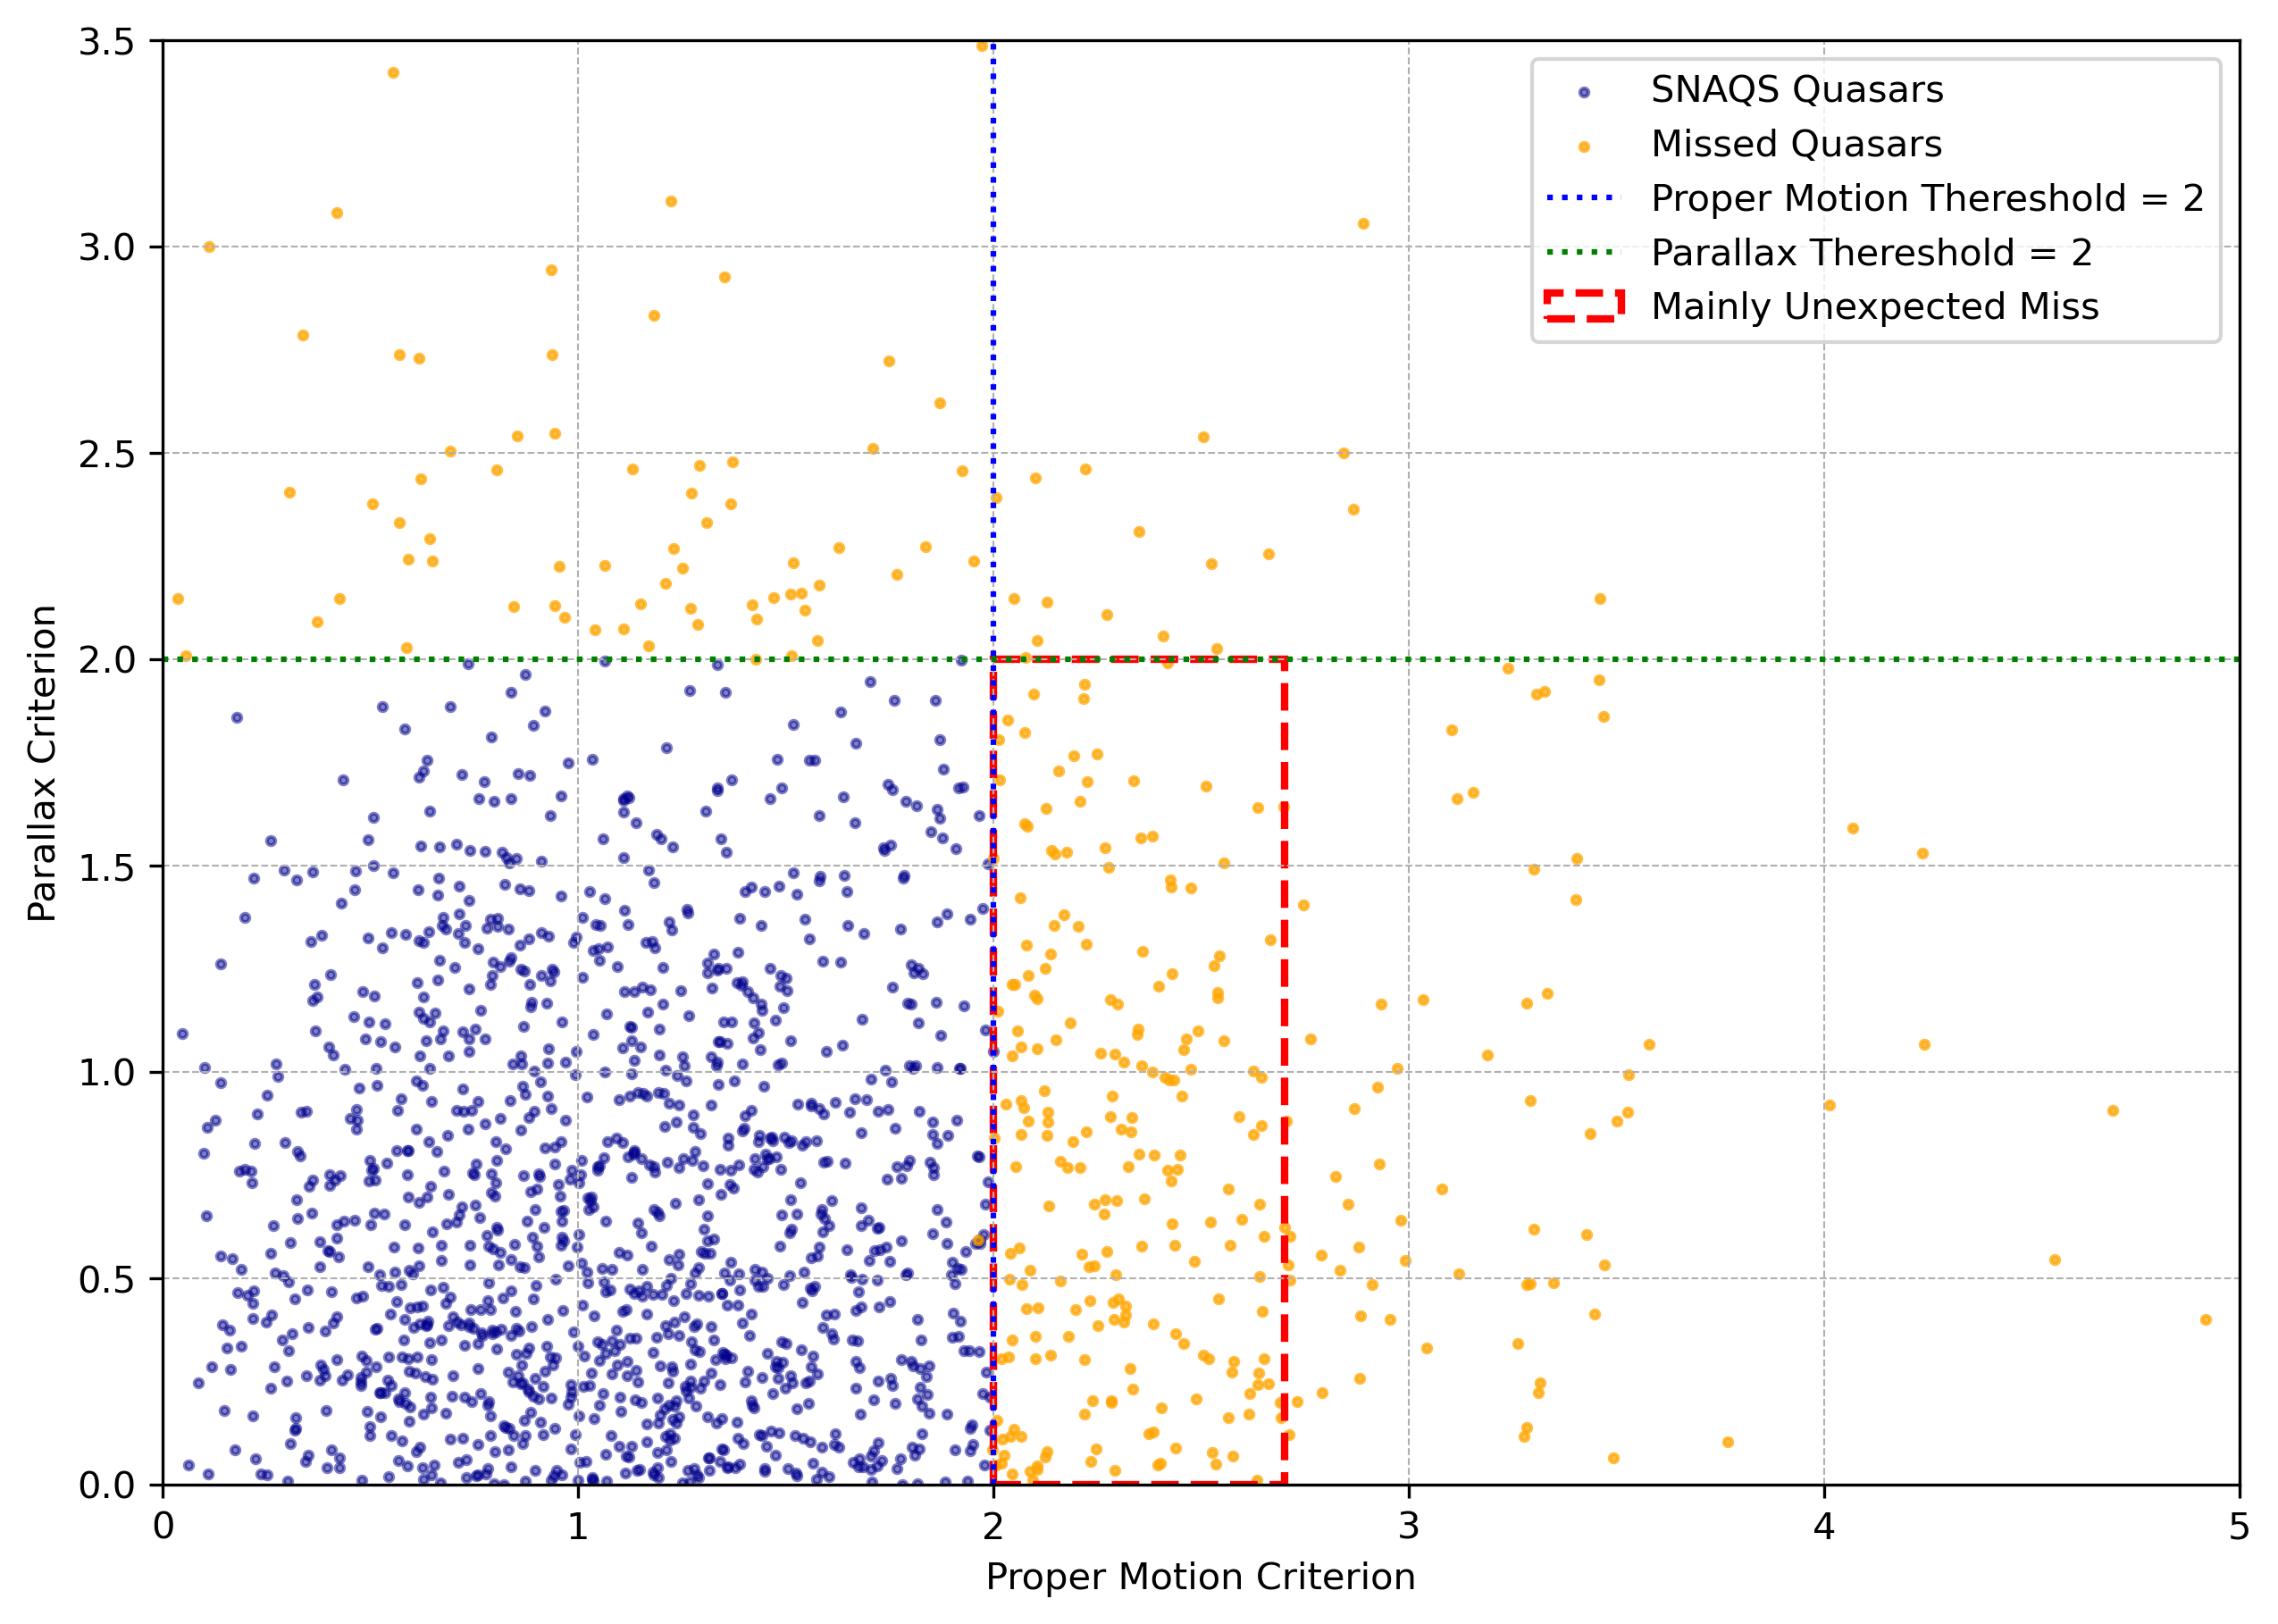
\includegraphics[width=0.85\linewidth]{figs//discuss/snaqs_missed_quasars.png}
    \caption{Distribution of Proper Motion and Parallax of Quasars in SDSS DR16Q in SNAQS area}
    \label{fig:snaqs_miss}
\end{figure}

We have found some reason that cause this issue and will discuss them in the following parts.

\section{About Astrometric Data from Gaia}

The selection of SNAQS and PAQS targets is mainly based on the Proper Motion and Parallax measurement results in Gaia EDR3 from \citet{gaiacollaborationGaiaEarlyData2021a}. But in the selection processing, the propagation of uncertainty of total proper motion was not fully correct, which made the selection result miss more candidates than expected. To clarify this, it is necessary to examine how the Gaia mission measures the proper motions of target objects.

\subsection{Proper Motion measurement in Gaia Mission} \label{sec:gaia_pm}

In \citet{lindegrenAstrometricCoreSolution2012}, authors provided the astrometric model for Gaia's measurements. The coordinate direction to the source $(i)$ at time $t$ is calculated with the "standard model", namely
\begin{equation}
    \bar{\boldsymbol{u}}_i(t) = \langle \boldsymbol{r}_i + (t_{\mathrm{B}} - t_{\mathrm{ep}})(\boldsymbol{p}_i \mu_{\alpha*i} + \boldsymbol{q}_i \mu_{\delta i} + \boldsymbol{r}_i \mu_{r i}) - \varpi_i \boldsymbol{b}_{\mathrm{G}}(t)/A_{\mathrm{u}} \rangle
\label{eq:cord-model}
\end{equation}
where the angular brackets signify vector length normalization, and $[\boldsymbol{p}_i\ \boldsymbol{q}_i\ \boldsymbol{r}_i]$ is the “normal triad” of the source with respect to the ICRS (International Celestial Reference System). In this triad, $\boldsymbol{r}_i$ is the barycentric coordinate direction to the source at time $t_{ep}$, $\boldsymbol{p}_i = \langle \boldsymbol{Z} \times \boldsymbol{r}_i \rangle$, and $\boldsymbol{q}_i = \boldsymbol{r}_i \times \boldsymbol{p}_i$. As a result, we got:
\begin{equation}
    \boldsymbol{p}_i \cdot \boldsymbol{q}_i=0
    \label{eq:pm-orth}
\end{equation}
which means that $\boldsymbol{p}_i$ and $\boldsymbol{q}_i$ are orthogonal. The total proper motion can be written as 
\begin{equation}
   \boldsymbol{\mu} = \boldsymbol{p}_i \mu_{\alpha*} + \boldsymbol{q}_i \mu_{\delta} 
   \label{eq:pm-model}
\end{equation}
This means $\mu_{\alpha*}$ and $\mu_{\delta}$ are two physical independent parameters.

In observation, we could compute the partial derivatives of Eq. \ref{eq:cord-model} as:
\begin{equation}
    \frac{\partial \bar{\boldsymbol{u}}_l}{\partial \mu_{\alpha*i}} = \boldsymbol{p}_i \tau_l \qquad \frac{\partial \bar{\boldsymbol{u}}_l}{\partial \mu_{\delta i}} = \boldsymbol{q}_i \tau_l
    \label{eq:pm-part}
\end{equation}
where $\tau_l = t_{Bl} - t_{ep}$. Combined with Eq. \ref{eq:pm-orth} and \ref{eq:pm-part}, it is easy to obtain the conclusion. In theory, the measurements on proper motion in two directions ($\mu_{\alpha*}, \mu_{\delta}$) are physically independent. If the measurement uncertainty contains, the proper motion in two directions of quasars should obey the standard normal distribution centered at zero in ideal condition.

To verify this conclusion, four quasar samples are selected. They are:
\begin{itemize}
    \item \textbf{SDSS DR16Q}: \textit{The Sloan Digital Sky Survey Quasar Catalog: Sixteenth Data Release} \citep{lykeSloanDigitalSky2020}
    \item \textbf{LAMOST Quasar Survey from Data Releases 2 to 11} \citep{dongLargeSkyArea2018, yaoLargeSkyArea2019, jinLargeSkyArea2023, lyuLargeSkyArea2025} 
    \item \textbf{Milliquas v8}: \textit{The Million Quasars (Milliquas) Catalogue, v8} \citep{fleschMillionQuasarsMilliquas2023}
    \item \textbf{LQAC-6}: \textit{Sixth Release of the Large Quasar Astrometric Catalogue} \citep{souchayLQAC6SixthRelease2024}
\end{itemize}
To minimize contamination in samples such as local Seyfert galaxies, only objects with $z>0.5$ are selected. The confirmed quasars from SDSS DR16Q and Milliquas v8 catalogues were cross-matched with Gaia DR3 astrometric data \citep{gaiacollaborationGaiaDataRelease2023} via the CDS cross-match service (Strasbourg), applying a distance threshold of \qty{1}{\arcsecond}. The astrometric parameters are identical to those in Gaia EDR3 \citep{vanleeuwenGaiaDR3Documentation2022}. In contrast, for the LAMOST Quasar Survey, the cross-match with Gaia DR3 data was performed using the \texttt{gaia\_source\_id} provided in the LAMOST catalogue. To avoid contamination from unresolved binaries, we excluded Gaia sources with $\mathrm{RUWE} \geq 1.4$, as recommended by \citet{fabriciusGaiaEarlyData2021}. Since the LQAC-6 catalogue was already cross-matched with Gaia data by \citet{souchayLQAC6SixthRelease2024}, we utilized its astrometric data directly. Following the data cleaning procedures, the number of confirmed quasars retained in each catalogue is:
\begin{itemize}
    \item \textbf{SDSS DR16Q}: \num{386478}
    \item \textbf{LAMOST Quasar Survey (DR2--DR11)}: \num{45619}
    \item \textbf{Milliquas v8}: \num{446956}
    \item \textbf{LQAC-6}: \num{433568}
\end{itemize}

We plotted the histograms of the proper motion-to-uncertainty ratios ($\mu_{\alpha*}/\sigma_{\mu_{\alpha*}}$ and $\mu_{\delta}/\sigma_{\mu_{\delta}}$) for the four samples. To robustly estimate the parameters of the underlying normal distribution while minimizing the influence of outliers, we applied a Median Absolute Deviation (MAD) fit. The resulting distributions and best-fit parameters are presented in Figure~\ref{fig:pm_dis} and Table~\ref{tab:pm_tab}, respectively.

\begin{figure}[htbp]
    \centering
    \begin{subfigure}[b]{0.48\textwidth}
        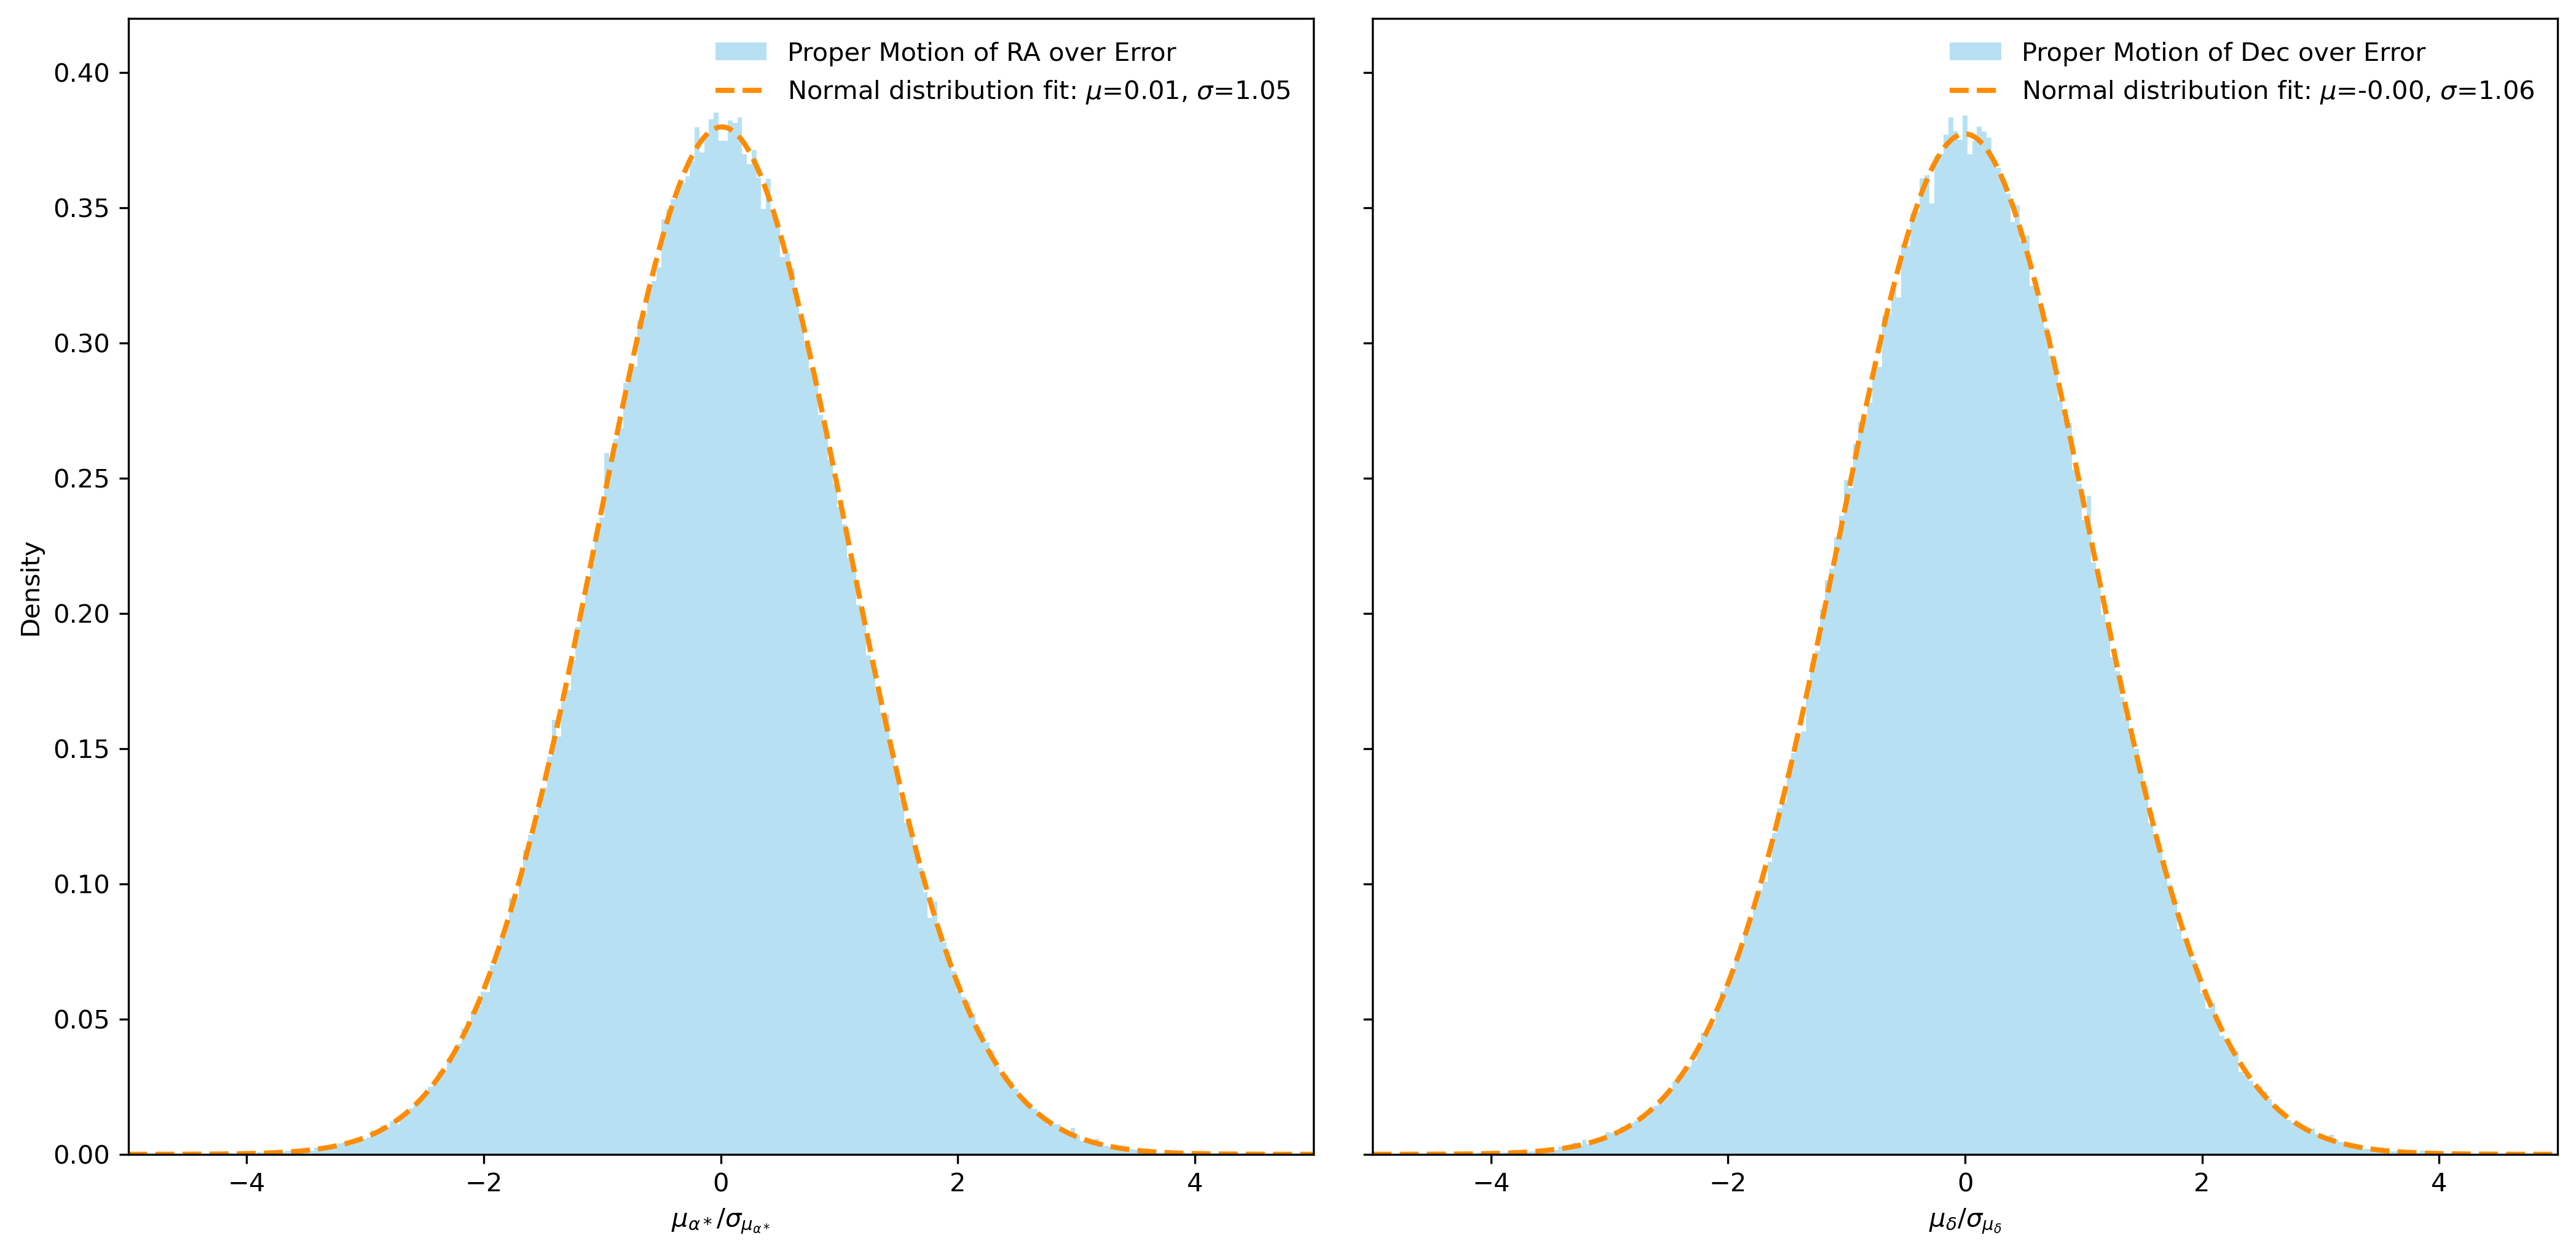
\includegraphics[width=\linewidth]{figs/discuss/sdss_qso_pm_significance.png}
        \caption{SDSS DR16Q}
        \label{fig:pm_sdss}
    \end{subfigure}
    \begin{subfigure}[b]{0.48\textwidth}
        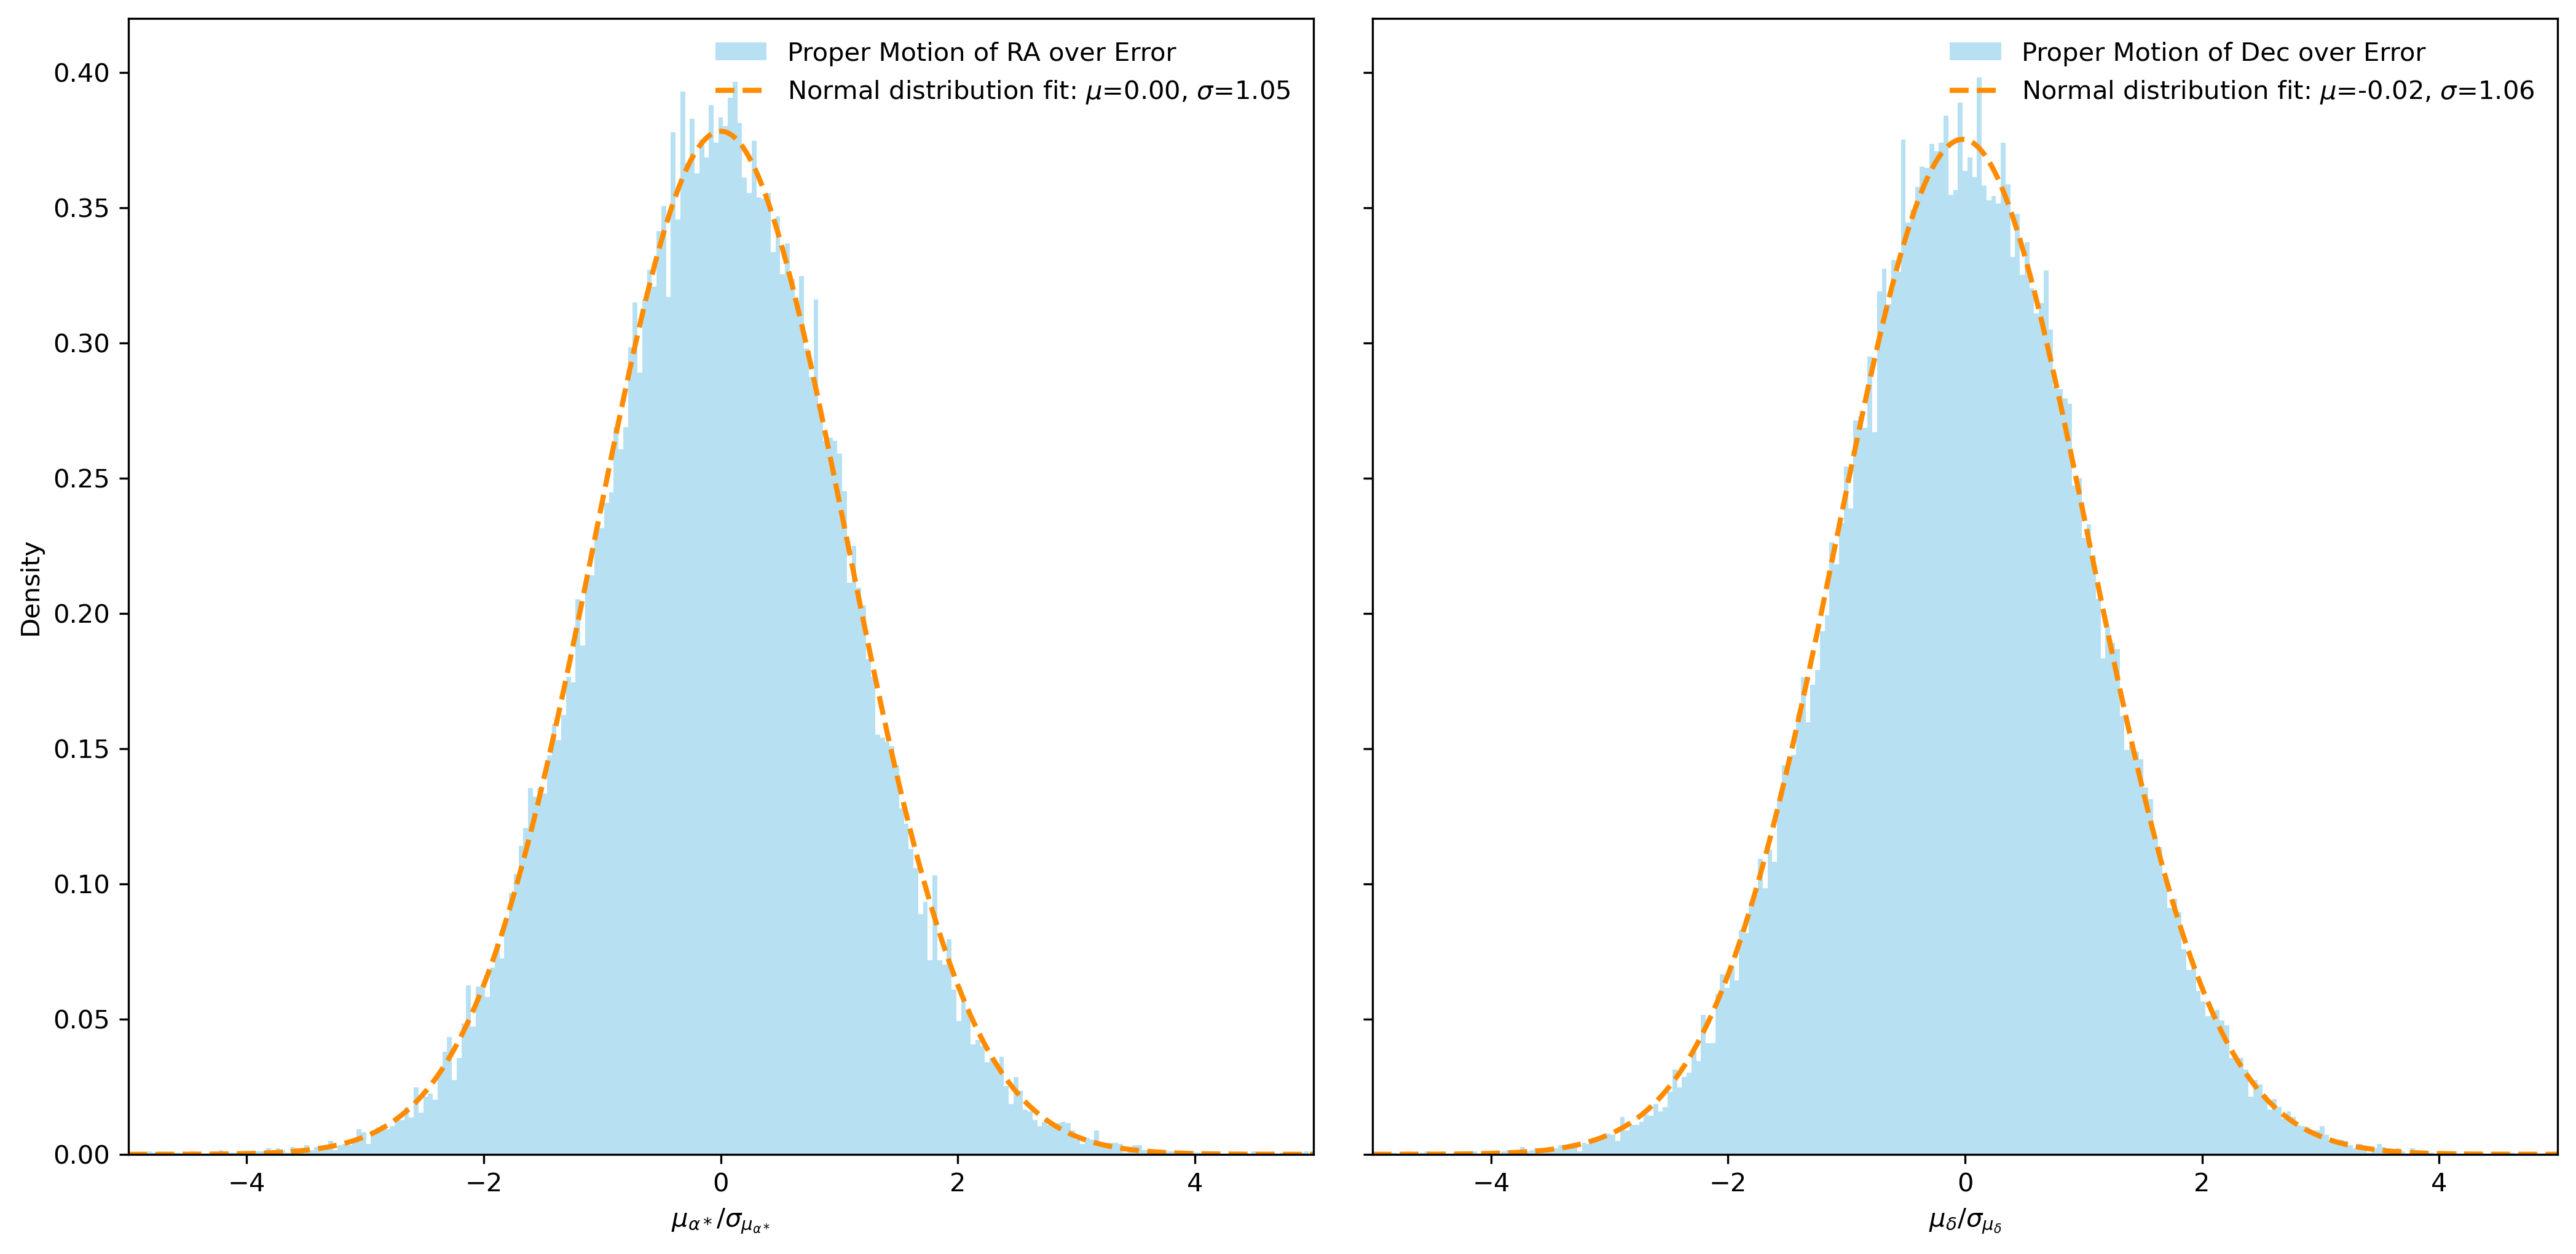
\includegraphics[width=\linewidth]{figs/discuss/lamost_qso_pm_significance.png}
        \caption{LAMOST Quasar Survey (DR2-11)}
        \label{fig:pm_lamost}
    \end{subfigure} \\
    \begin{subfigure}[b]{0.48\textwidth}
        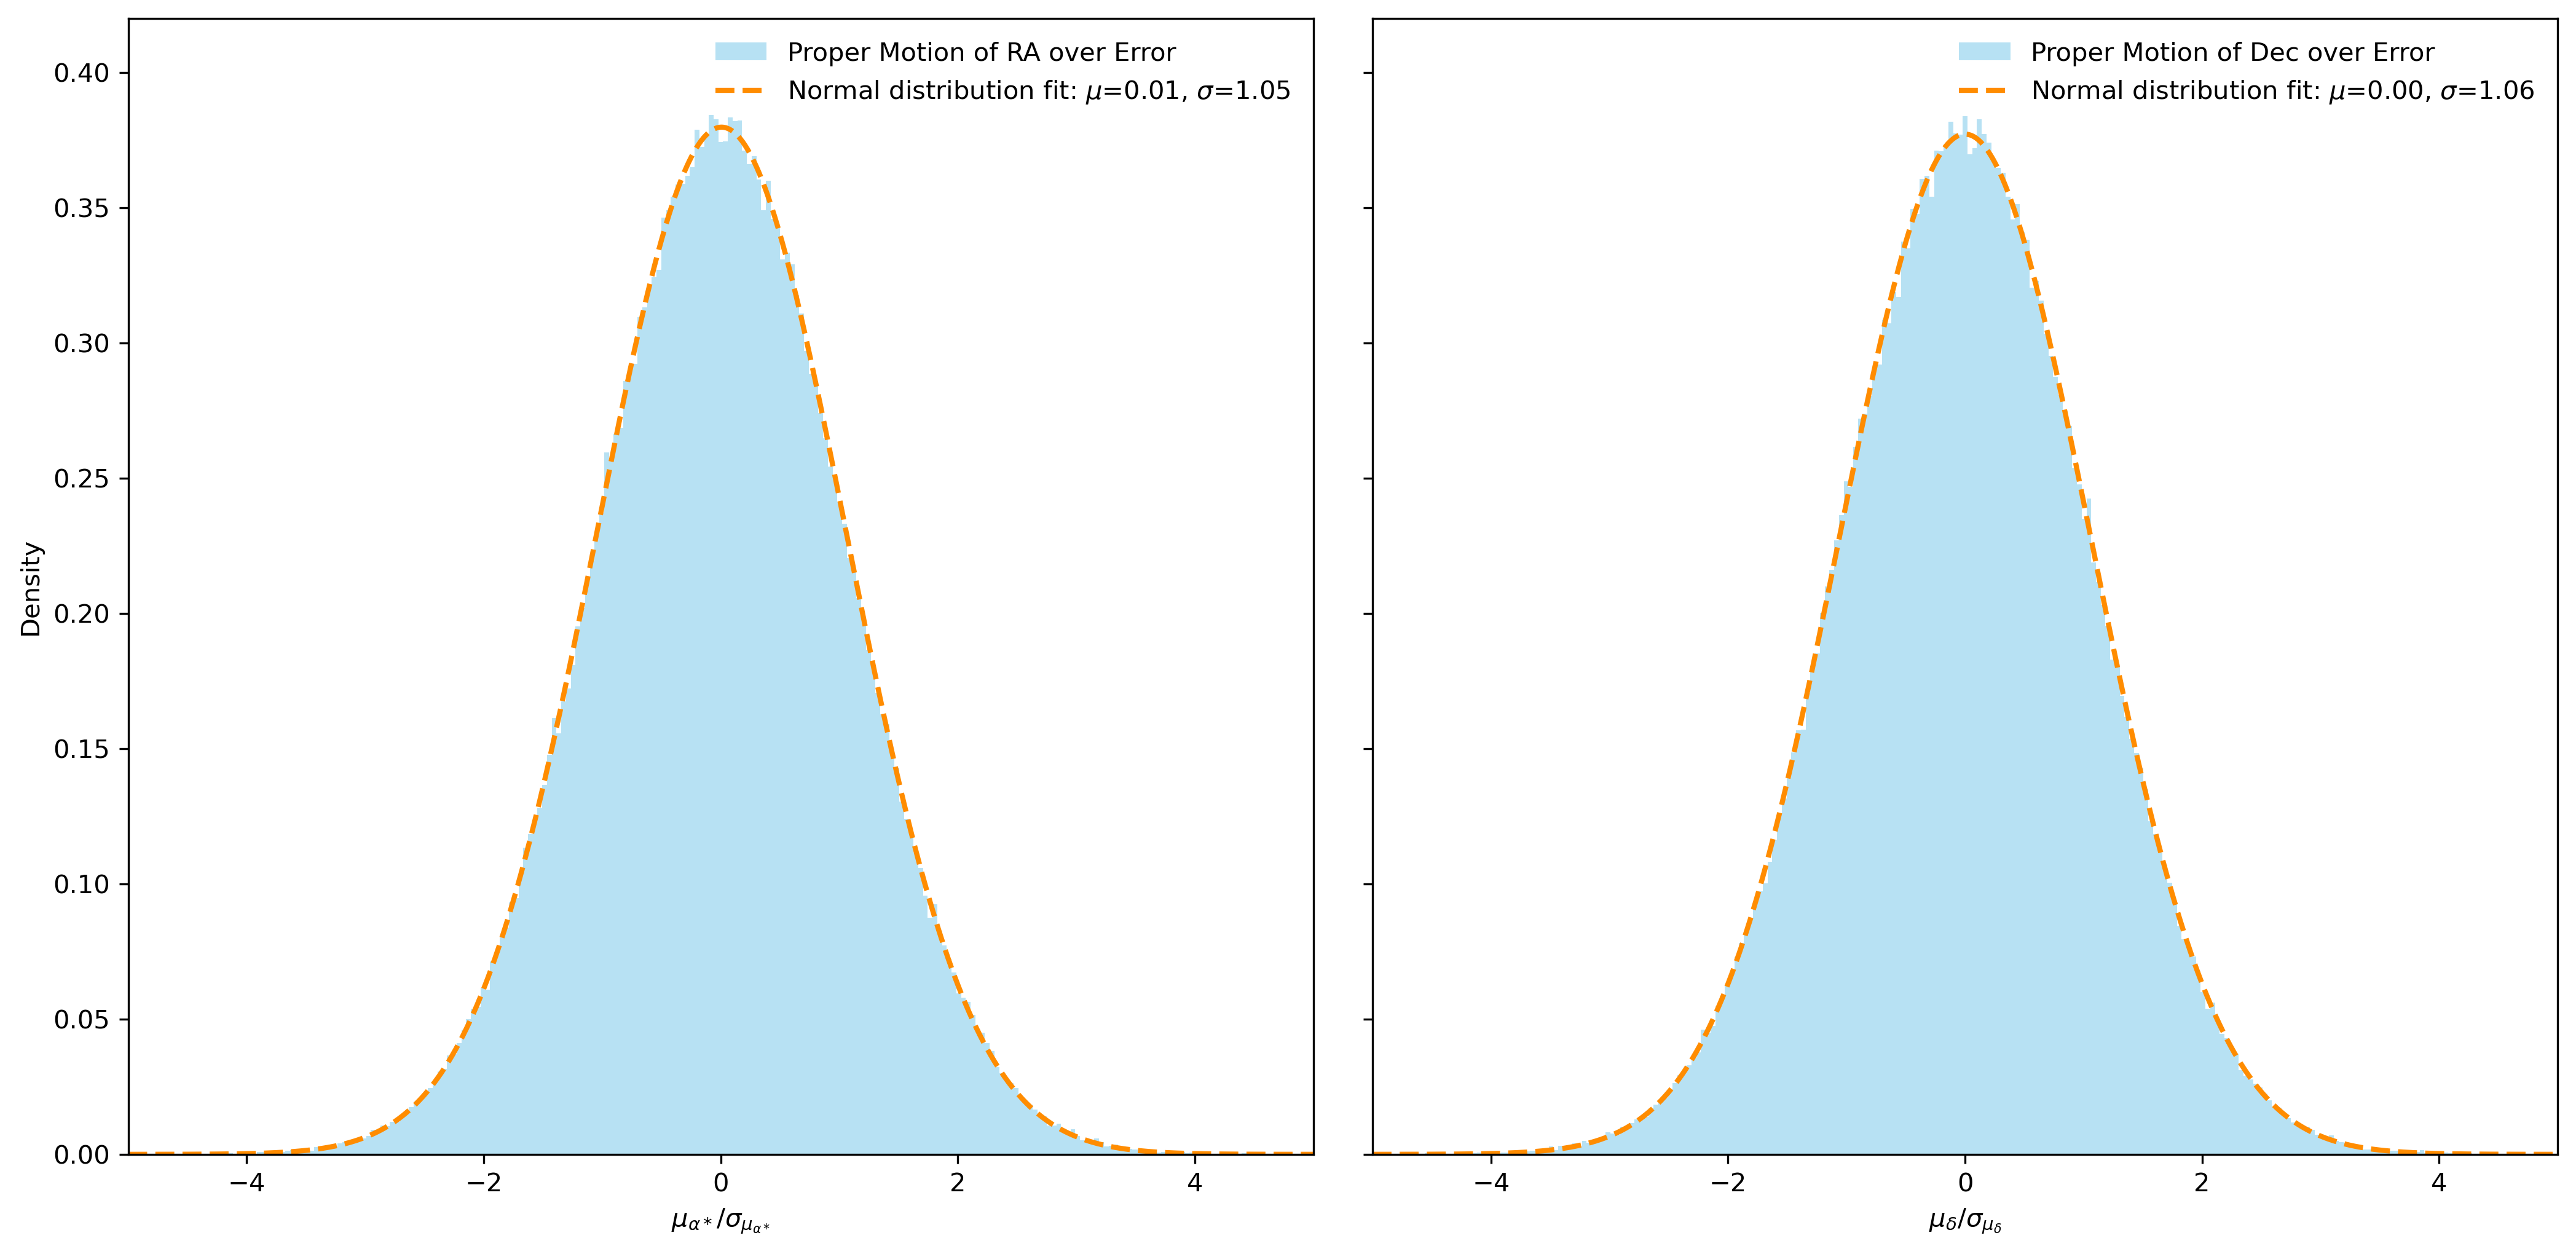
\includegraphics[width=\linewidth]{figs/discuss/milliquas_qso_pm_significance.png}
        \caption{Milliquas v8}
        \label{fig:pm_milliquas}
    \end{subfigure} 
    \begin{subfigure}[b]{0.48\textwidth}
        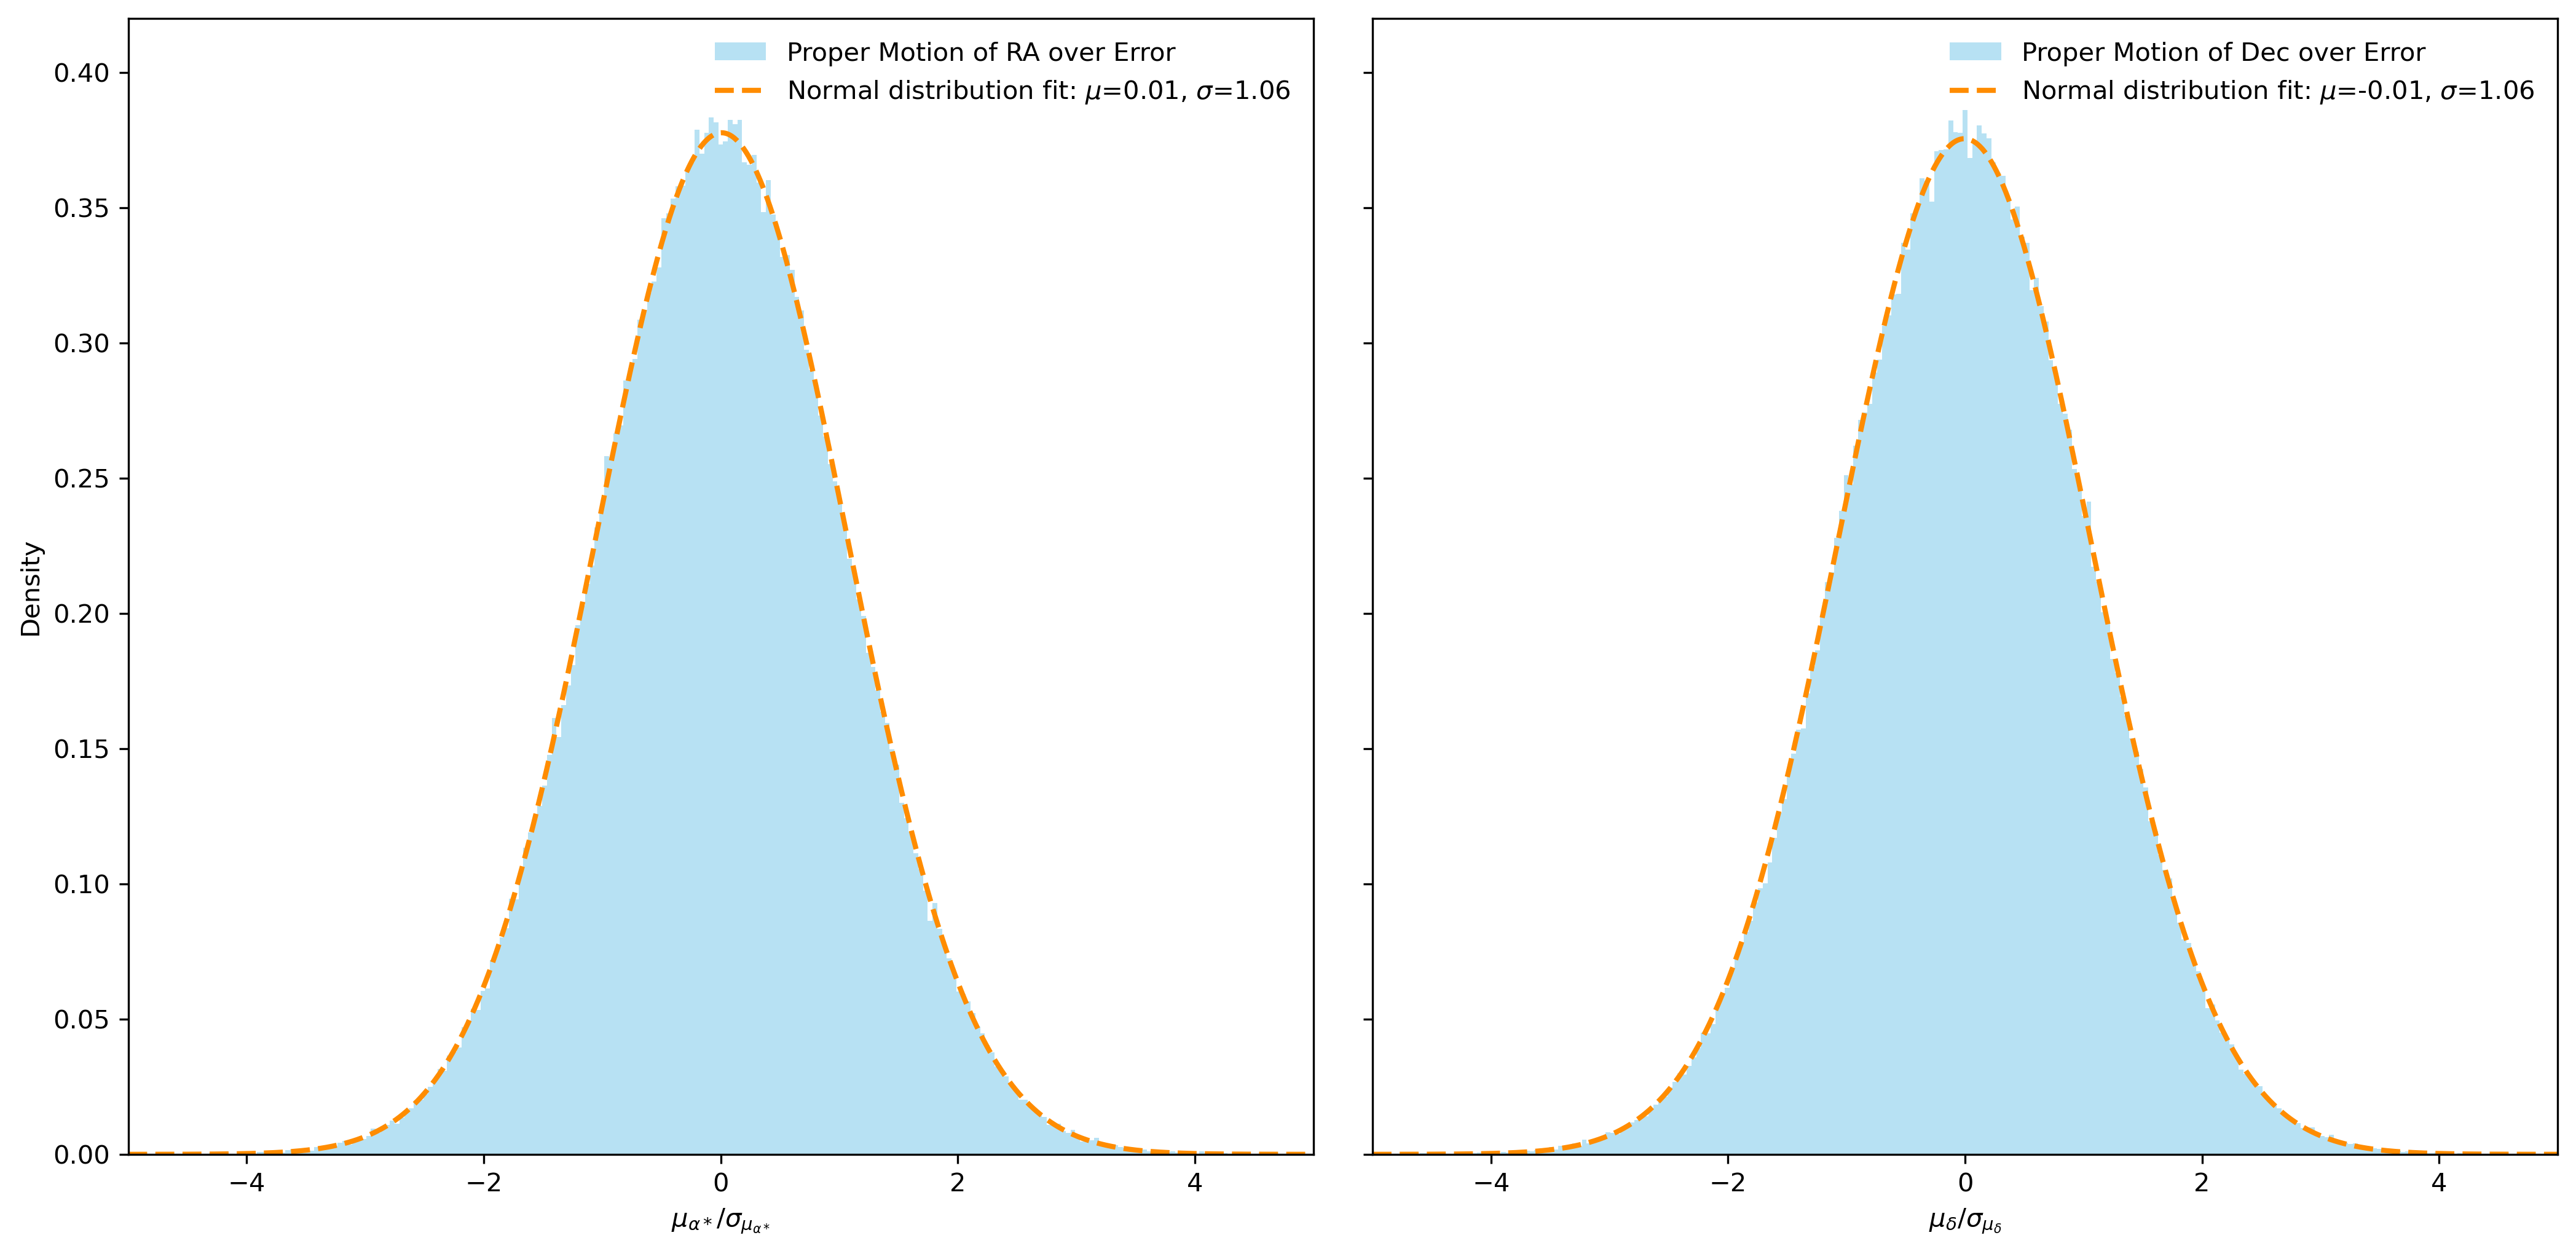
\includegraphics[width=\linewidth]{figs/discuss/lqac6_qso_pm_significance.png}
        \caption{LQAC-6}
        \label{fig:pm_lqac6}
    \end{subfigure} 
    \caption{Distributions of the proper motion-to-uncertainty ratios ($\mu_{\alpha*}/\sigma_{\mu_{\alpha*}}$ and $\mu_{\delta}/\sigma_{\mu_{\delta}}$) across the four evaluated quasar catalogues. The orange dashed lines indicate the robust normal distribution fits obtained via MAD. As illustrated, the empirical data are well-described by these Gaussian profiles.}
    \label{fig:pm_dis}
\end{figure}

\begin{table}[htbp]
    \centering
    \begin{tabular}{l c c c c}
        \toprule
        \multirow{2}{*}{Samples} & \multicolumn{2}{c}{$\mu_{\alpha*}/\sigma_{\mu_{\alpha*}}$} & \multicolumn{2}{c}{$\mu_{\delta}/\sigma_{\mu_{\delta}}$} \\
        \cmidrule(lr){2-3} \cmidrule(lr){4-5}
        & $\mu$ & $\sigma$ & $\mu$ & $\sigma$ \\
        \midrule
        \textbf{SDSS DR16Q} & 0.009  & 1.050 & -0.002 & 1.057 \\
        \textbf{LAMOST Quasar Survey (DR2--11)} & 0.000 & 1.055 & -0.021 & 1.063 \\
        \textbf{Milliquas v8} & 0.007 & 1.050 & 0.000 & 1.058 \\
        \textbf{LQAC-6} & 0.007 & 1.056 & -0.006 & 1.062 \\
        \bottomrule
    \end{tabular}
    \caption{The Parameters of fitted Gaussian Distribution for the proper motion-to-uncertainty ratios ($\mu_{\alpha*}/\sigma_{\mu_{\alpha*}}$ and $\mu_{\delta}/\sigma_{\mu_{\delta}}$) across the four evaluated quasar catalogues}
    \label{tab:pm_tab}
\end{table}

These results demonstrate that the proper motion-to-uncertainty ratios are well-described by Gaussian profiles, which is in excellent agreement with theoretical predictions. The slightly broadened standard deviations of our fits ($\sigma \approx 1.05$--$1.07$‬) are perfectly consistent with the findings of \citet{fabriciusGaiaEarlyData2021}, who demonstrated that astrometric uncertainties in the Gaia EDR3 catalogue tend to be underestimated.

\subsection{About the statistic distribution of total proper motion}

In the selection of SNAQS and PAQS, the criterion of proper motion is the value of standard deviations for which the proper motion of the objects deviates from zero. This  $(S/N)_{\mu_{total}}$ is from the following formula:
\begin{equation}
    (S/N)_{\mu_{total}} = \sqrt{\left(\frac{\mu_{\alpha*}}{\sigma_{\mu_{\alpha*}}}\right)^2 + \left(\frac{\mu_{\delta}}{\sigma_{\mu_{\delta}}}\right)^2}
    \label{eq:sn_pm_old}
\end{equation}

We proceed to evaluate the statistical distribution of this criterion in theory and practice. As established in Section \ref{sec:gaia_pm}, $\mu_{\alpha*} / \sigma_{\mu_{\alpha*}}$ and $\mu_{\delta} / \sigma_{\mu_{\delta}}$ can be theoretically treated as two independent standard normal variables. While our original selection process we approximated ${(S/N)}_{\mu_{total}}$ as a normal variable to estimate the number of missing candidates, this non-linear combination inherently prevents a normal distribution. In fact, ${(S/N)}_{\mu_{total}}$ follows Rayleigh Distribution. The Rayleigh distribution describes the magnitude of a two-dimensional vector whose orthogonal components follow independent, zero-mean normal distributions (further mathematical details are outlined in Appendix~\ref{app:rayleigh}).

\begin{figure}[htbp]
    \centering
    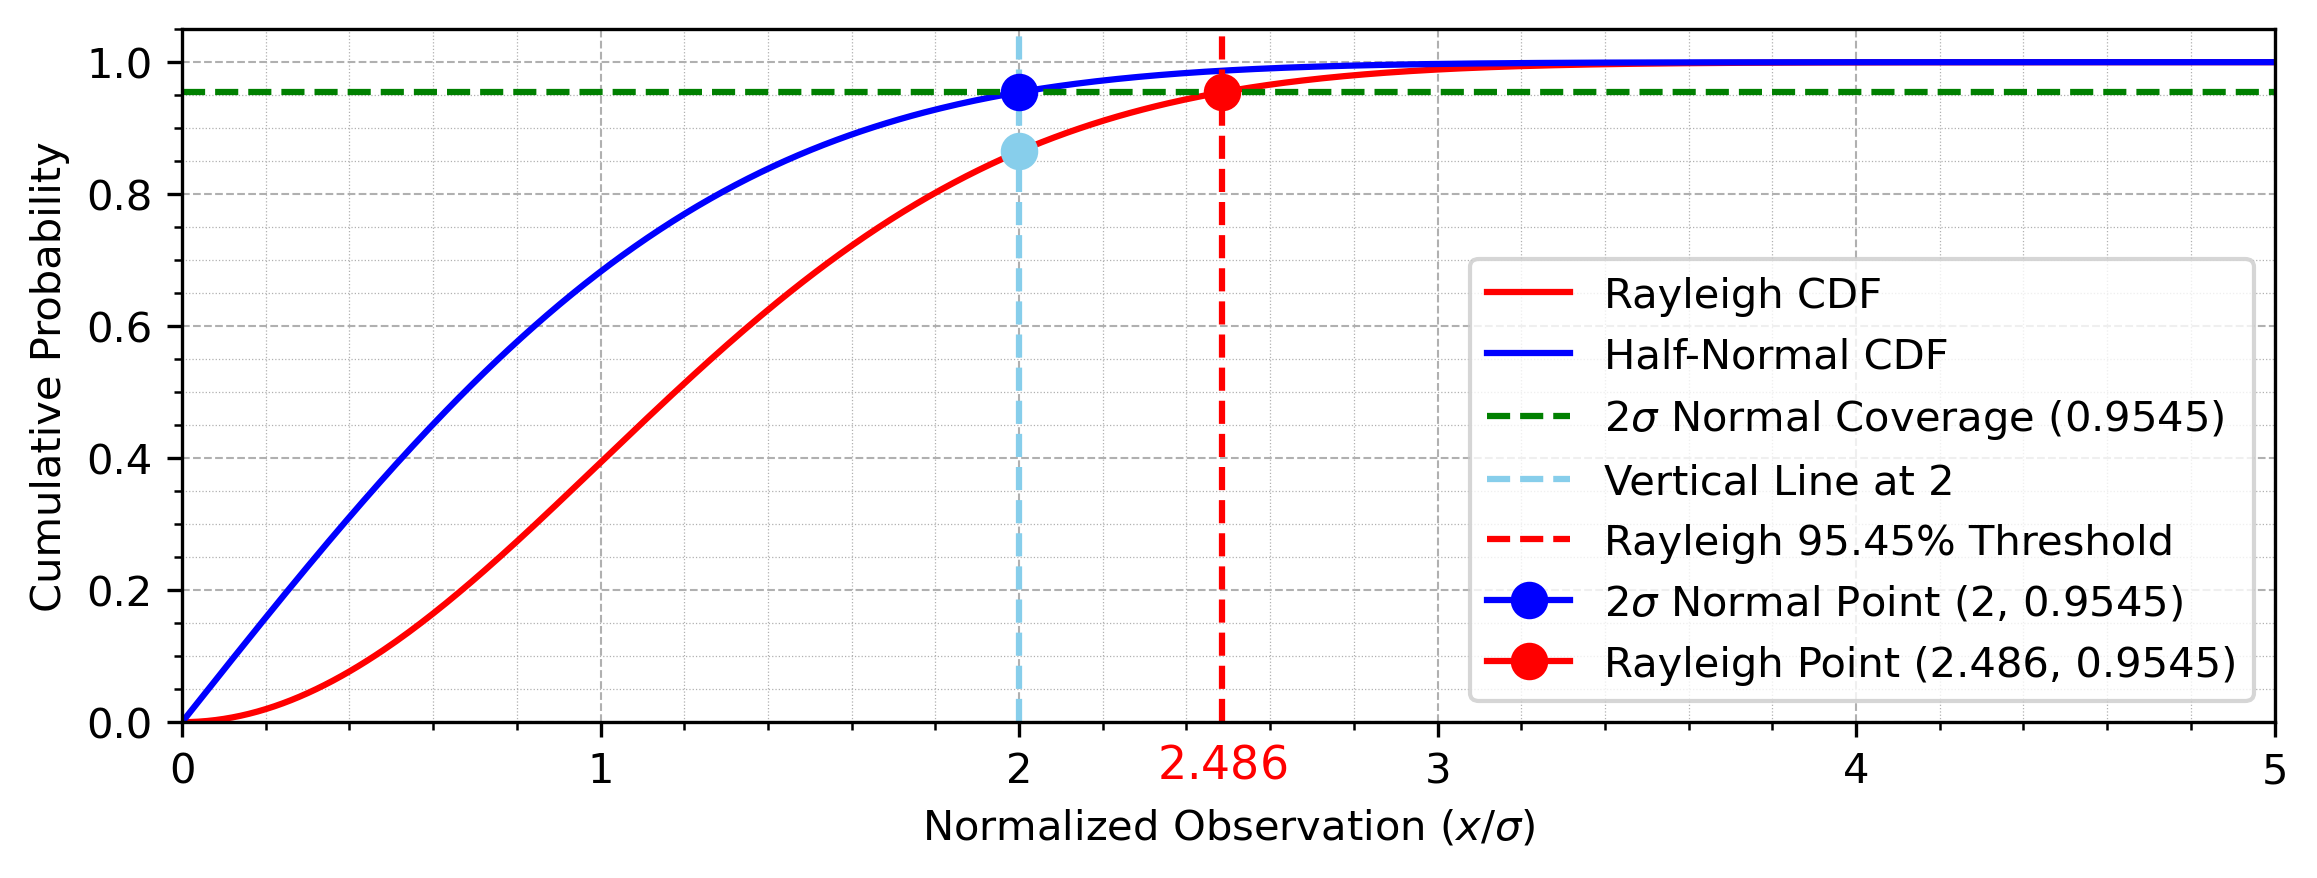
\includegraphics[width=\linewidth]{figs//discuss/rayleigh_halfnorm_cdf.png}
    \caption{CDFs of Half Normal and Rayleigh Distribution with scale parameters as 1. The green dashed line shows the probability of measurements fall in $\pm 2\sigma$ in a standard normal distribution.}
    \label{fig:ray_norm_cdf}
\end{figure}

For a standard normal distribution, approximately \qty{95.45}{\percent} of the values fall within the $\pm 2\sigma$ interval,  corresponding to an expected miss rate of \qty{4.55}{\percent}. Figure~\ref{fig:ray_norm_cdf} compares the cumulative distribution functions (CDFs) of these two distributions. If we apply a threshold of 2 to the Rayleigh distribution, it captures only about \qty{86.47}{\percent} of the measurements (an approximate \qty{13.53}{\percent} miss rate), resulting in a data loss nearly three times higher than expected. Consequently, a larger threshold is required to retain a similar proportion of the data.

\begin{figure}[htbp]
    \centering
    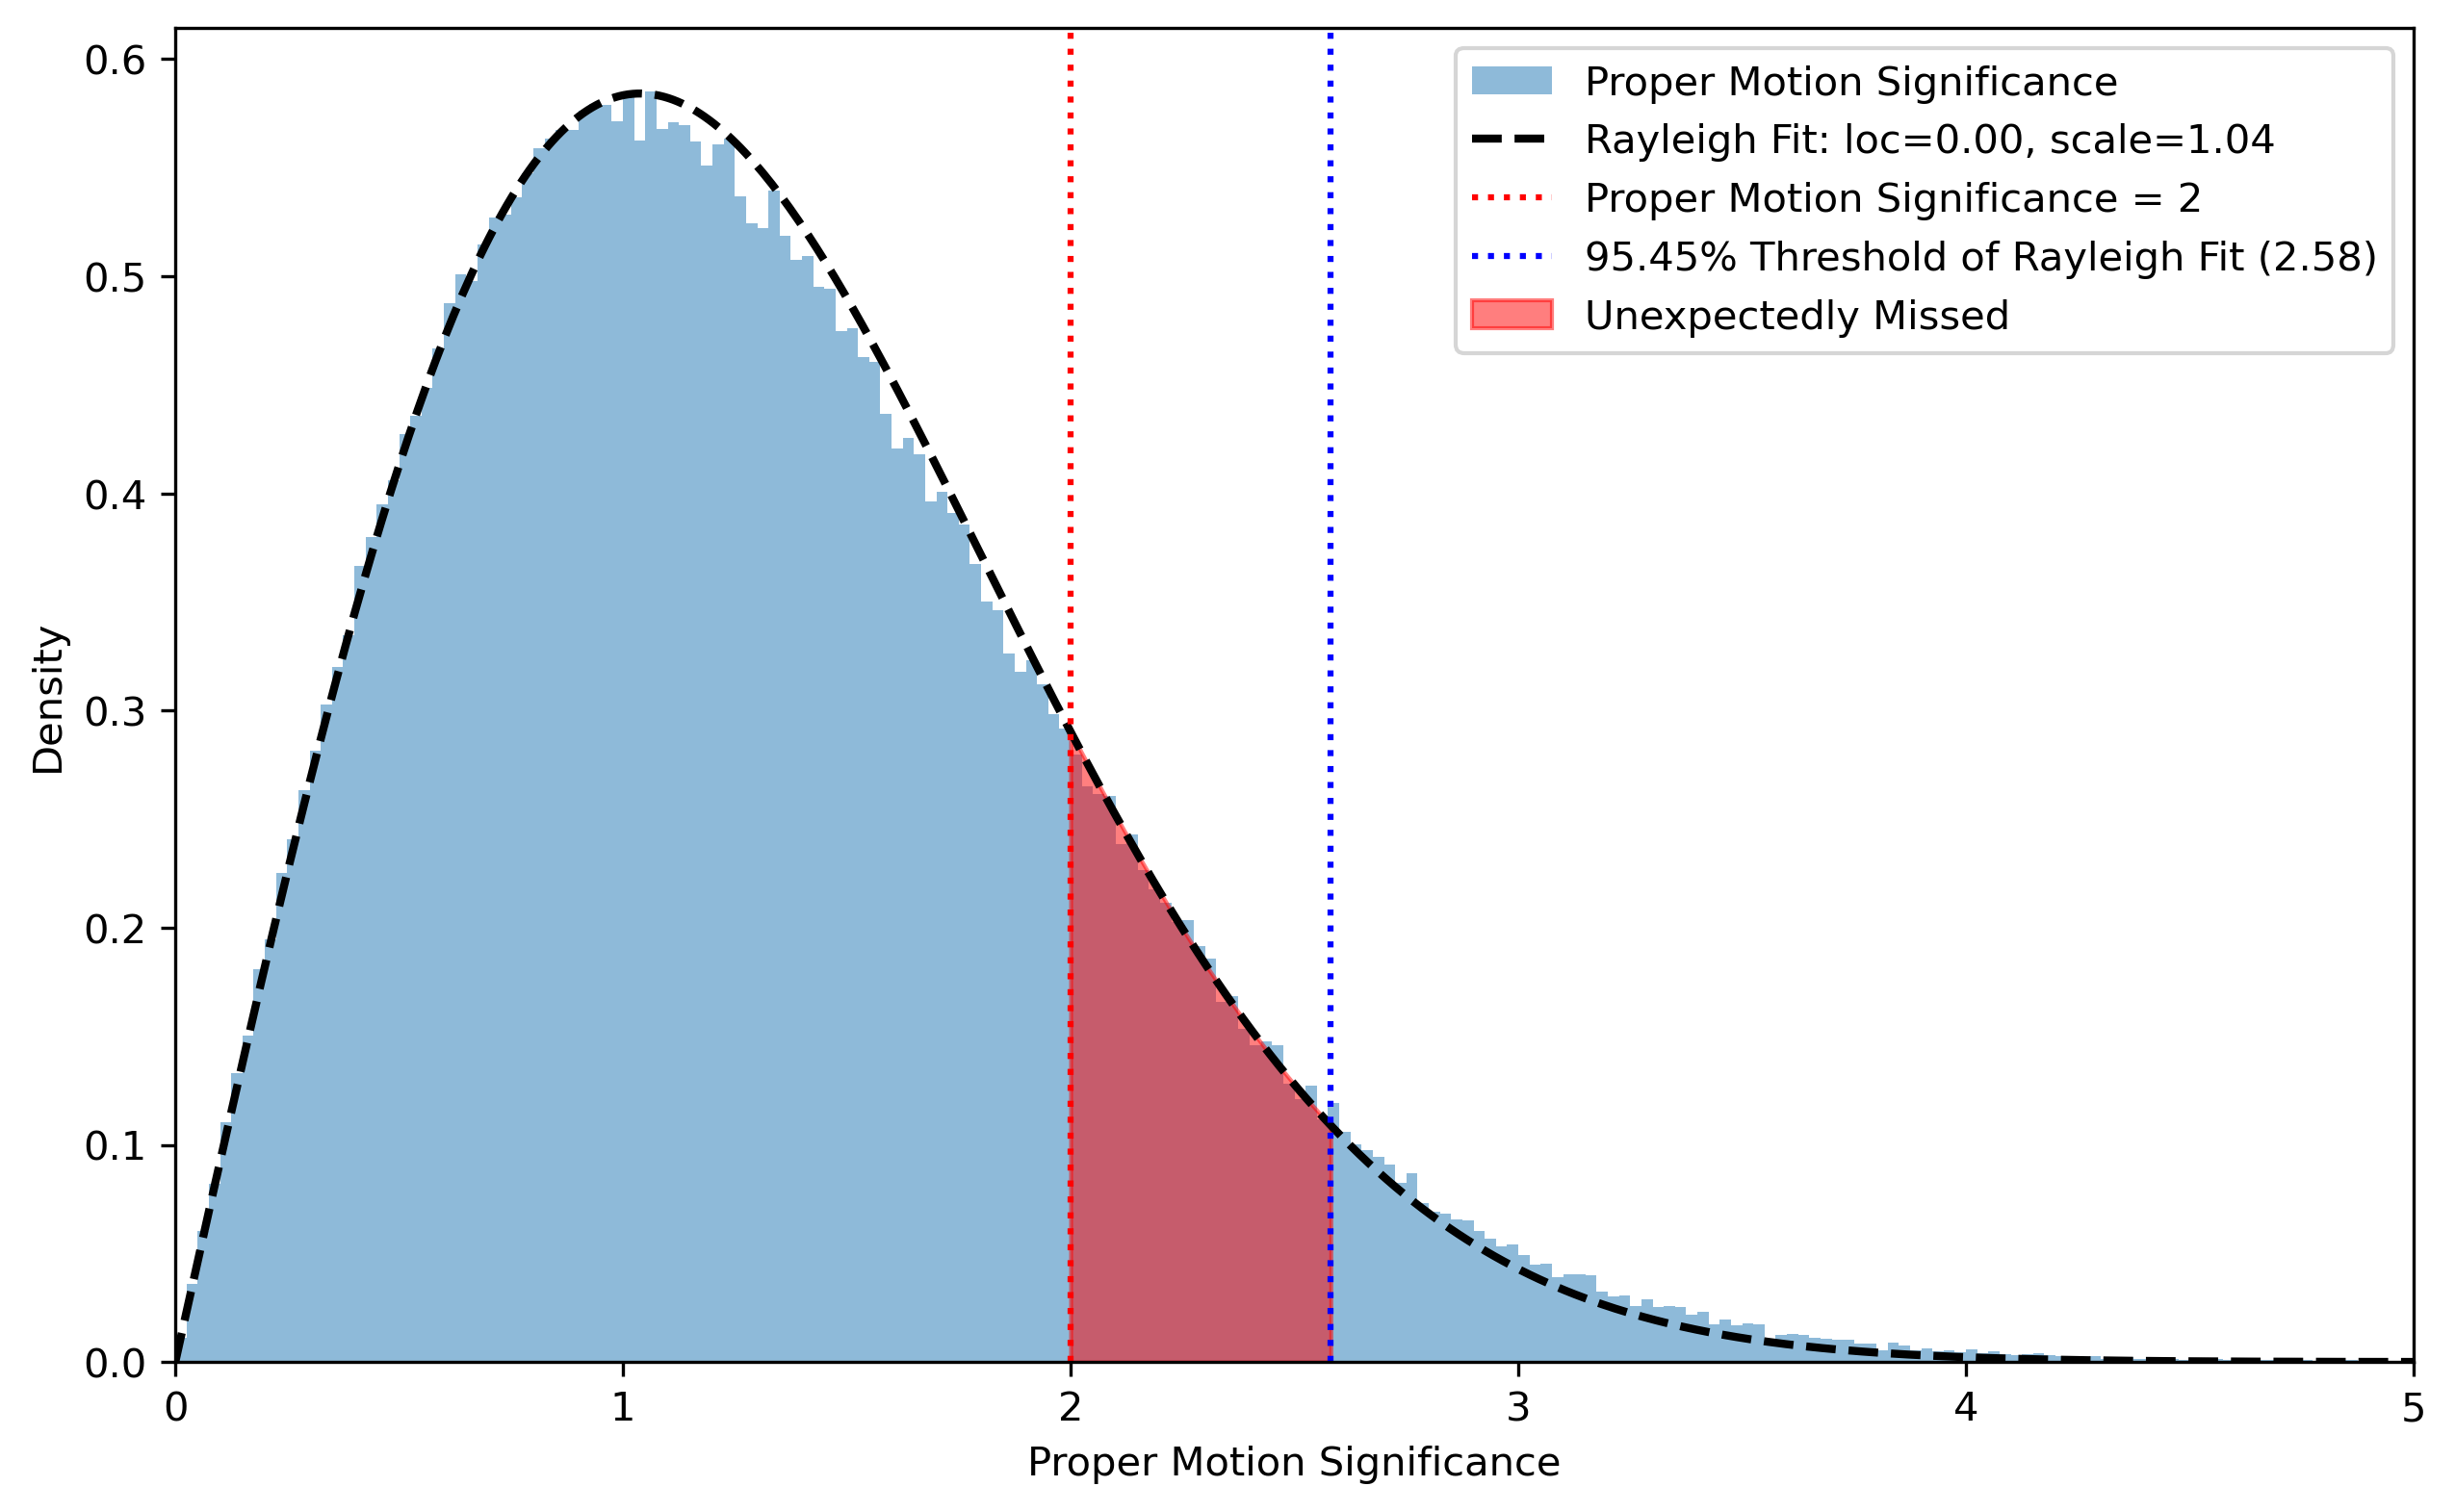
\includegraphics[width=0.9\linewidth]{figs/discuss/sdss_qso_pm_significance_rayleigh_fit.png}
    \caption{Distribution of the total proper motion criterion for the SDSS DR16Q sample. The solid black line represents the best-fit Rayleigh distribution, while the red shaded area highlights the fraction of candidates excluded when adopting a threshold of 2.}
    \label{fig:sdss_qso_ray}
\end{figure}

In practical observations, due to the underestimation of proper motion uncertainties, the scale parameter of the actual distribution exceeds 1. By fitting a Rayleigh distribution to the SDSS DR16Q catalogue, we derived a scale parameter of $\sigma \approx 1.04$, consistent with the discussion in Section~\ref{sec:gaia_pm}. Under these empirical conditions, applying a threshold of 2 yields a capture rate of only \qty{83.36}{\percent}. This translates to an approximate \qty{15.64}{\percent} miss rate, which is nearly four times ($\approx 3.44$ times) higher than the theoretical expectation.

\subsection{Error propagation of total proper motion in the combination of proper motion in RA and Dec}
\label{sec:error_prop}

Although the method as Equation~\ref{eq:sn_pm_old} is effective in detecting apparent motion against the celestial background, its application is largely limited to finding objects with high proper motion or removing objects in background. 

In the selection of quasar candidates, this formula is not accurate enough. To calculate the uncertainty with higher precision, we should begin from the method to get the total proper motion. The total proper motion could be written as Equation \ref{eq:pm_tot}:
\begin{equation}
    \mu_{total}=\sqrt{{\mu_{\alpha*}}^2+{\mu_{\delta}}^2}
    \label{eq:pm_tot}
\end{equation}

For a multivariable function $f(x,y)$, according to the first-order error propagation formula, the variance of $f(x,y)$ is:
\[\sigma_f^2 = \left( \frac{\partial f}{\partial x} \right)^2 \sigma_x^2 + \left( \frac{\partial f}{\partial y} \right)^2 \sigma_y^2 + 2 \left( \frac{\partial f}{\partial x} \right) \left( \frac{\partial f}{\partial y} \right) \text{cov}(x, y)\]
Theoretically, the measurement of proper motion in RA and Dec are independent from each other, the uncertainty of total proper motion can be written as:
\begin{equation}
    \sigma_{\mu_{total}} = \sqrt{ \left(\frac{\mu_{\alpha*}}{\mu_{total}}\right)^2 {\sigma^2_{\mu_{\alpha*}}} + \left(\frac{\mu_{\delta}}{\mu_{total}}\right)^2 {\sigma^2_{\mu_{\delta}}}} = \frac{1}{\mu_{total}} \sqrt{{\mu_{\alpha*}}^2 {\sigma^2_{\mu_{\alpha*}}} + {\mu_{\delta}}^2 {\sigma^2_{\mu_{\delta}}}}
\end{equation}

But in practical observation, the proper motion measurements in RA and Dec are not completely independent. In Gaia EDR3 table there is a column named \texttt{pmra\_pmdec\_corr}, which is the correlation between proper motion in right ascension and proper motion in declination. 

\begin{figure}[htbp]
  \centering
  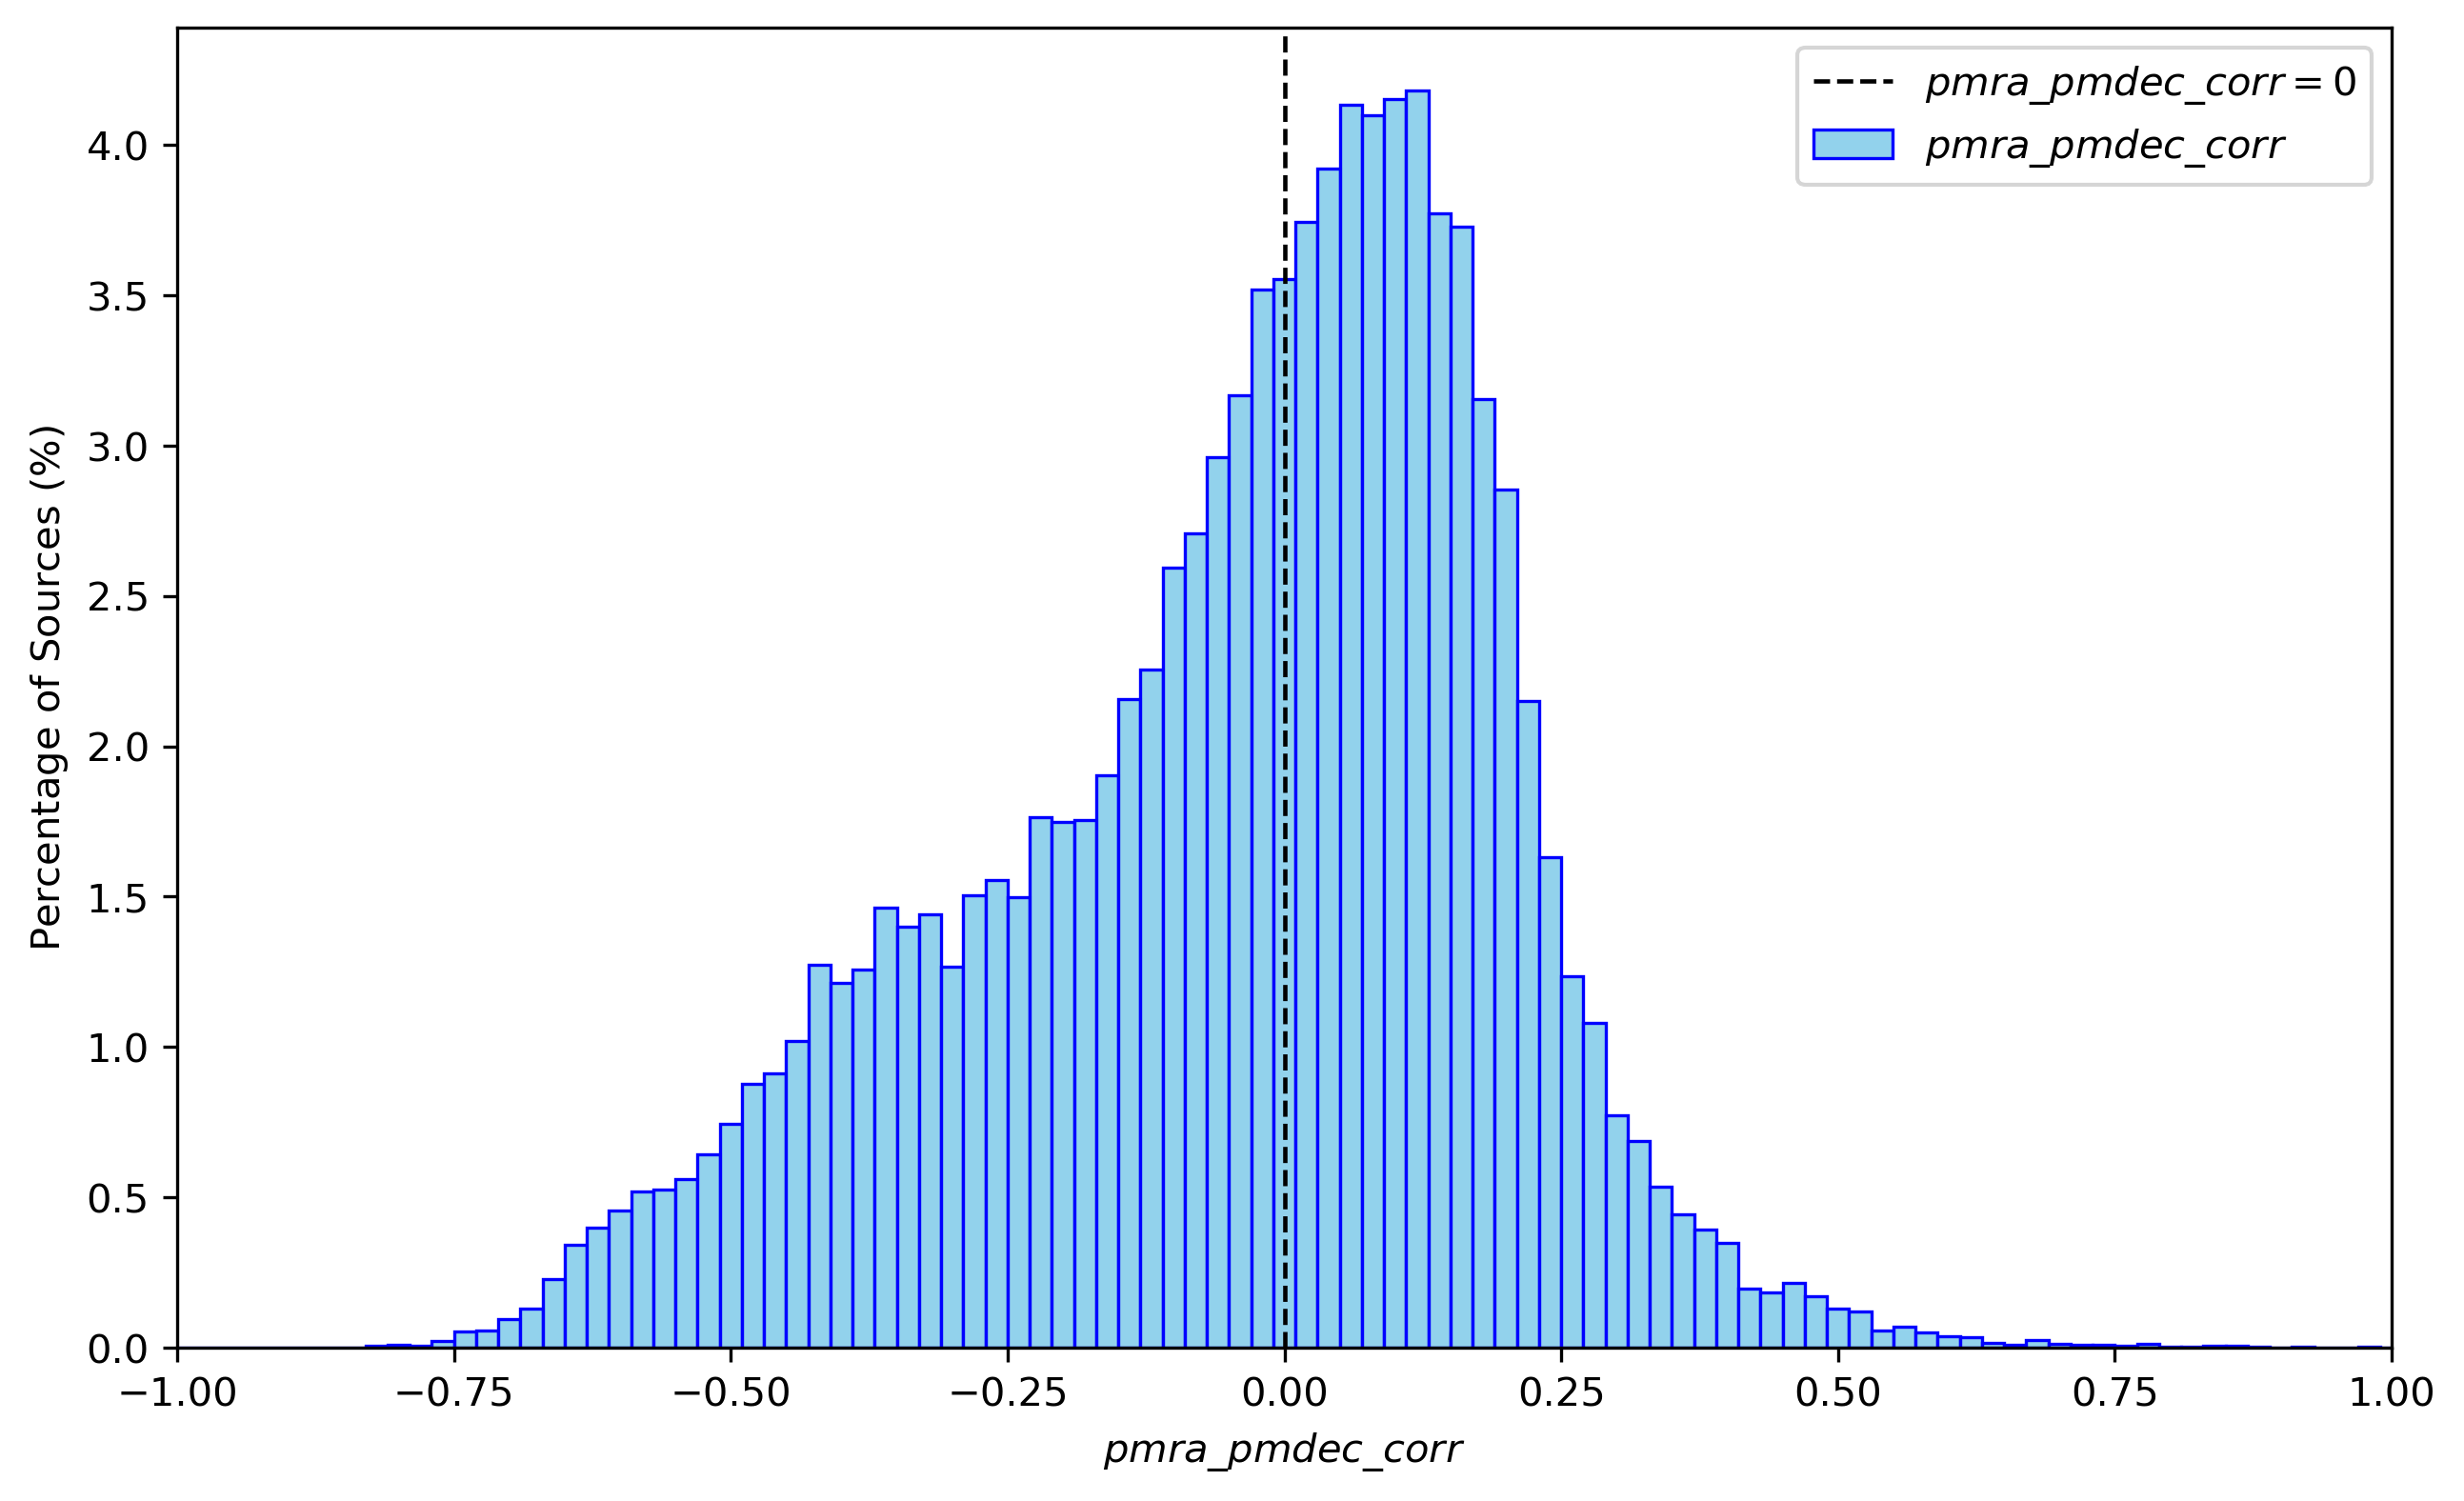
\includegraphics[width=0.9\linewidth]{figs/discuss/pm_correlation_histogram.png}
  \caption{This histogram is the distribution of \texttt{pmra\_pmdec\_corr}, the correlation between proper motion in right ascension and proper motion in declination. It shows that the correlation is not able to be ignored}
  \label{fig:pmra_pmdec_corr_dist}
\end{figure}

We checked all \texttt{pmra\_pmdec\_corr} values of available sources bright enough ($\text{Gmag}>19$) and low parallax (be zero in $2\sigma$) in SNAQS area from Gaia EDR3 Data. It contains \num{45675} targets in this sample. Figure \ref{fig:pmra_pmdec_corr_dist} shows the statistical distribution of the values.

In this sample, only \num{1622} ($\approx \qty{3.55}{\percent}$) targets have an irreducible correlation value (absolute value less than 0.01). As a result, the uncertainty must contain the correlation part: 
\[2 \left( \frac{\partial f}{\partial x} \right) \left( \frac{\partial f}{\partial y} \right) \text{cov}(x, y)= 2\mu_{\alpha*}\mu_{\delta}\rho_{\mu_{\alpha*}\mu_{\delta}}\sigma_{\mu_{\alpha*}}\sigma_{\mu_{\delta}}.\] 
A more accurate uncertainty can be written as Equation \ref{eq:pm_sig_corr}.
\begin{equation}
    \sigma_{\mu_{total}}=\frac{1}{\mu_{total}}\sqrt{{{\mu_{\alpha*}}^2\sigma^2_{\mu_{\alpha*}}}+{{{\mu_{\delta}}^2\sigma^2_{\mu_{\delta}}}+2\rho_{\mu_{\alpha*}\mu_{\delta}}\mu_{\alpha*}\mu_{\delta}\sigma_{\mu_{\alpha*}}\sigma_{\mu_{\delta}}}}
    \label{eq:pm_sig_corr}
\end{equation}
The criterion ${(S/N)}_{\mu_{total}}$ became:
\begin{equation}
    {(S/N)}_{\mu_{total}, corrected} = \frac{\mu_{total}}{\sigma_{\mu_{total}}}=\frac{{\mu_{total}}^2}{\sqrt{{{\mu_{\alpha*}}^2\sigma^2_{\mu_{\alpha*}}}+{{{\mu_{\delta}}^2\sigma^2_{\mu_{\delta}}}+2\rho_{\mu_{\alpha*}\mu_{\delta}}\mu_{\alpha*}\mu_{\delta}\sigma_{\mu_{\alpha*}}\sigma_{\mu_{\delta}}}}}
    \label{eq:sn_pm_new}
\end{equation}

I also calculated the relative deviation $\delta$ between the result of Equation \ref{eq:sn_pm_old} and Equation \ref{eq:sn_pm_new} for this 45,675 target sample:
\[\delta = \frac{{(S/N)}_{\mu_{total}, uncorrected}-{(S/N)}_{\mu_{total}, corrected}}{{(S/N)}_{\mu_{total}, corrected}}\] 

\begin{figure}[htbp]
  \centering
  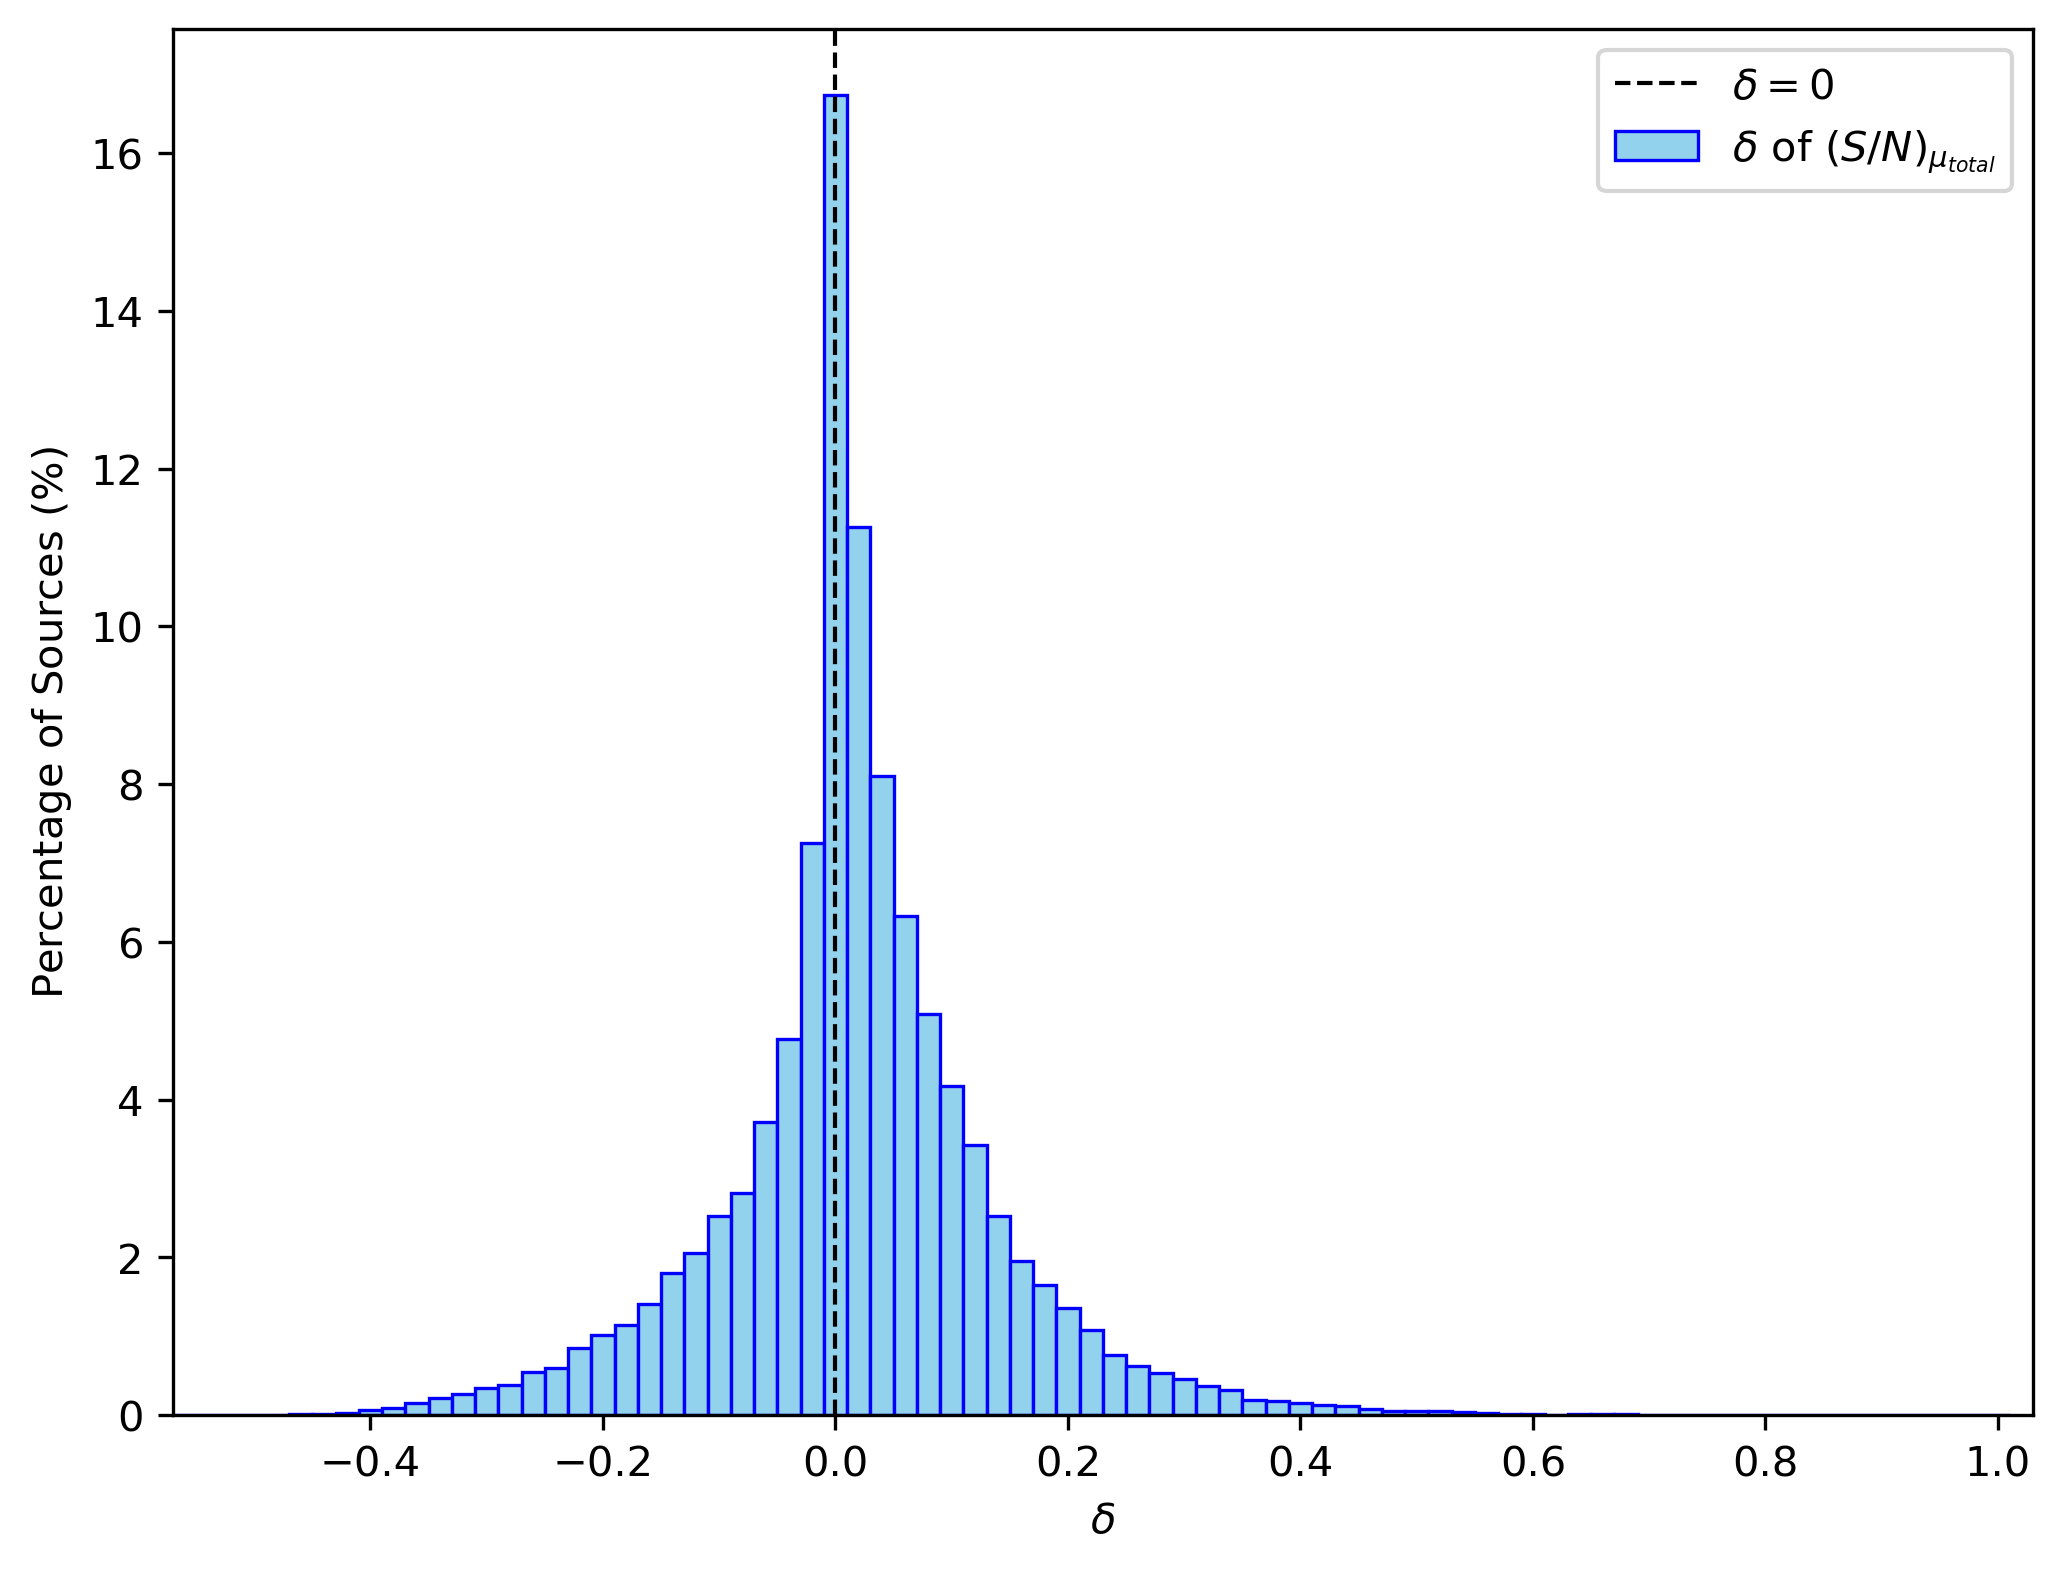
\includegraphics[width=0.9\linewidth]{figs/discuss/pm_significance_difference_histogram.png}
  \caption{This histogram is the distribution of $\delta$, the relative deviation of the total proper motion divided by its standard error which from two different methods.}
  \label{fig:pm_delta_dist}
\end{figure}

Figure~\ref{fig:pm_delta_dist} presents the comparison results for this sample. We find that the criterion of total proper motion is over-estimated for \num{27499} ($\approx \qty{60.2}{\percent}$) targets in this sample. In contrast, the discrepancy is negligible (relative deviation $< \qty{1}{\percent}$) for only \num{7644} targets ($\approx \qty{16.7}{\percent}$). 

Therefore, as discussed above, the difference of uncertainty propagation is non-negligible in practical processing. 

\subsection{Two-Dimensional Proper Motion Analysis}

While the previous section addressed the uncertainty of individual components, proper motion is measured as a two-dimensional vector on the celestial sphere. Also, we discussed how the proper motion is measured in \ref{sec:gaia_pm}. To comprehensively evaluate the astrometric behaviour of our targets, we could extend this uncertainty analysis to two-dimensional space. 

As illustrated in Figure~\ref{fig:separated_legend}, under the ideal assumption that the proper motion measurements in the two directions are statistically independent, our selection can be visualised as identifying targets whose normalized proper motions ($\mu_{\alpha*}/\sigma_{\mu_{\alpha*}}$, $\mu_{\delta}/\sigma_{\mu_{\delta}}$) fall within the circular $2\sigma$ boundary (black circle). However, in practical astrometry, the correlation between the two components is non-negligible. This covariance transforms the selection area into an error ellipse, whose shape and orientation depend directly on the correlation coefficient. For a better explanation, we plot the $2\sigma$ boundary when covariance are $\pm0.5$, $0.98$ (highest value in sample data at \ref{sec:error_prop}) and $-0.83$ (lowest value in the same sample data).

\begin{figure}[htbp]
    \centering
    \begin{minipage}[t]{0.65\linewidth}
        \vspace{0pt}
        \centering
        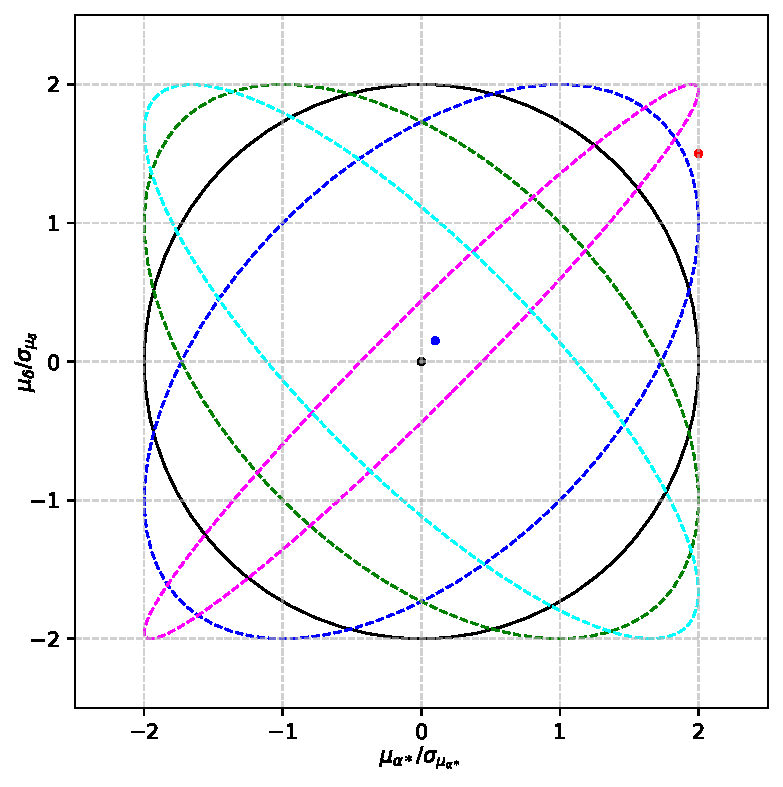
\includegraphics[width=\linewidth]{figs/discuss/error_ellipses.pdf}
    \end{minipage}% 
    \hfill 
    \begin{minipage}[t]{0.3\linewidth}
        \centering
        \vspace{0pt}
        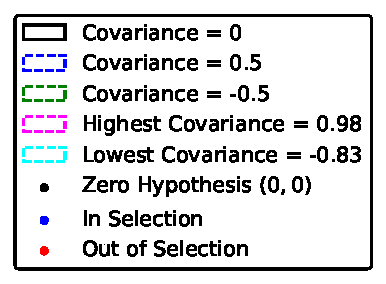
\includegraphics[width=\linewidth]{figs/discuss/legend_only.pdf}
        \vspace{1.5em}
        \captionof{figure}{$2\sigma$ error ellipses for the zero hypothesis. It shows how the correlation coefficients influence the $2\sigma$ area size and shape. (The range of covariance value is from the same sample in \ref{sec:error_prop}.)}
        \label{fig:separated_legend}
    \end{minipage}
\end{figure}

\section{A New Method for Selection of Quasar Candidates by Only Astrometric Data}

Fundamentally, our selection criterion is based on measuring the statistical distance of the proper motion from the null hypothesis ($\boldsymbol{\mu} = \boldsymbol{0}$). Our proposed method will continue to build upon this framework.

\subsection{Hypothesis Testing and Mahalanobis Distance}
The previous criterion (Eq.~\ref{eq:sn_pm_old}) is mathematically equivalent to calculating the Euclidean distance in the normalized parameter space:
\begin{equation}
    D_{E(\boldsymbol{x},\boldsymbol{y})} = \sqrt{(\boldsymbol{x}-\boldsymbol{y})^2} \implies D_{E(\mu)} = \sqrt{\left(\frac{\mu_{\alpha*}}{\sigma_{\mu_{\alpha*}}}\right)^2 + \left(\frac{\mu_{\delta}}{\sigma_{\mu_{\delta}}}\right)^2}
    \label{eq:e_dist}
\end{equation}

However, this Euclidean approach assumes that the measurements are fully independent and neglects the cross-correlation between the two proper motion components. To rigorously account for the covariance, the Mahalanobis distance is the optimal metric. It is generally defined as:
\begin{equation}
    D_{M(\boldsymbol{x},\boldsymbol{y})} = \sqrt{(\boldsymbol{x}-\boldsymbol{y})^T \Sigma^{-1}(\boldsymbol{x}-\boldsymbol{y})}
    \label{eq:m_dist}
\end{equation}
where $\Sigma$ represents the covariance matrix. 

For selection, we could set $\boldsymbol{x}=(\mu_{\alpha*}, \mu_{\delta})$ and null hypothesis $\boldsymbol{y}=(0,0)$. The distance is:
\begin{equation}
    D_{M(\mu)}=\sqrt{(\mu_{\alpha*}, \mu_{\delta})^T\Sigma^{-1}(\mu_{\alpha*}, \mu_{\delta})}, \quad \Sigma=
    \begin{pmatrix}
    \sigma^2_{\mu_{\alpha*}} & \rho_{\mu_{\alpha*}\mu_{\delta}} \sigma_{\mu_{\alpha*}} \sigma_{\mu_{\delta}}  \\
    \rho_{\mu_{\alpha*}\mu_{\delta}} \sigma_{\mu_{\alpha*}} \sigma_{\mu_{\delta}} & \sigma^2_{\mu_{\delta}}
    \end{pmatrix}
    \label{eq:m_dist_pm}
\end{equation}

Theoretically, the squared Mahalanobis Distance follows the chi-squared distribution with $k$ degrees of freedom. In our two-dimensional proper motion space, $k=2$. By substituting the covariance matrix into Eq.~\ref{eq:m_dist_pm}, we obtain the squared Mahalanobis distance:

\begin{equation}
    D^2_{M(\mu)} = \frac{1}{1-\rho^2_{\mu_{\alpha*}\mu_{\delta}}} \left[ \left(\frac{\mu_{\alpha*}}{\sigma_{\mu_{\alpha*}}}\right)^2 + \left(\frac{\mu_{\delta}}{\sigma_{\mu_{\delta}}}\right)^2 - 2\rho_{\mu_{\alpha*}\mu_{\delta}} \left(\frac{\mu_{\alpha*}}{\sigma_{\mu_{\alpha*}}}\right) \left(\frac{\mu_{\delta}}{\sigma_{\mu_{\delta}}}\right) \right]
    \label{eq:m_dist_sq}
\end{equation}

Consequently, we can evaluate the $p$-value of the null hypothesis ($\boldsymbol{\mu} = (0,0)$) by calculating the survival function ($1-\mathrm{CDF}$) of the $\chi^2_2$ distribution with $k=2$ using the result from Eq.~\ref{eq:m_dist_sq}. Obviously, Mahalanobis Distance is a dimensionless value.

To validate the effectiveness of our proposed method, we constructed three distinct reference samples—comprising galaxies, stars, and quasars—for comparative analysis. The galaxy and stellar samples were sourced from SDSS DR17 catalog \citep{abdurroufSeventeenthDataRelease2022}, relying on the automatic spectroscopic classifications provided in the catalog. The quasar sample was derived from the SDSS DR16Q catalog \citep{lykeSloanDigitalSky2020}, which contains visually inspected and confirmed quasars. After cross-matching these datasets with Gaia DR3 using a search radius of \qty{1}{\arcsecond} and removing the sources with only $3p$ solutions, our final reference samples consist of:
\begin{itemize}
    \item Galaxies in SDSS DR17: \num{54035} objects
    \item Stars in SDSS DR17: \num{615304} objects
    \item Quasars in SDSS DR16Q: \num{146794} objects
\end{itemize}

We measure the Squared Mahalanobis Distance of these three samples and obtain the distribution as Fig~\ref{fig:m_dist_sq}. In this figure, we could find quasars and galaxies following the 2 degree-of-freedom $\chi^2$ distribution as distant sources. At the same time, star sample are located uniformly along the x-axis. However, it's also significant that the standard $\chi^2$ distribution cannot perfectly fit the result due to multiple issues in practical measurements. We will try to fix it in sections after. Discussion in this section will be based only on the ideal 2 degree-of-freedom $\chi^2$ distribution.

\begin{figure}[htbp]
    \centering
    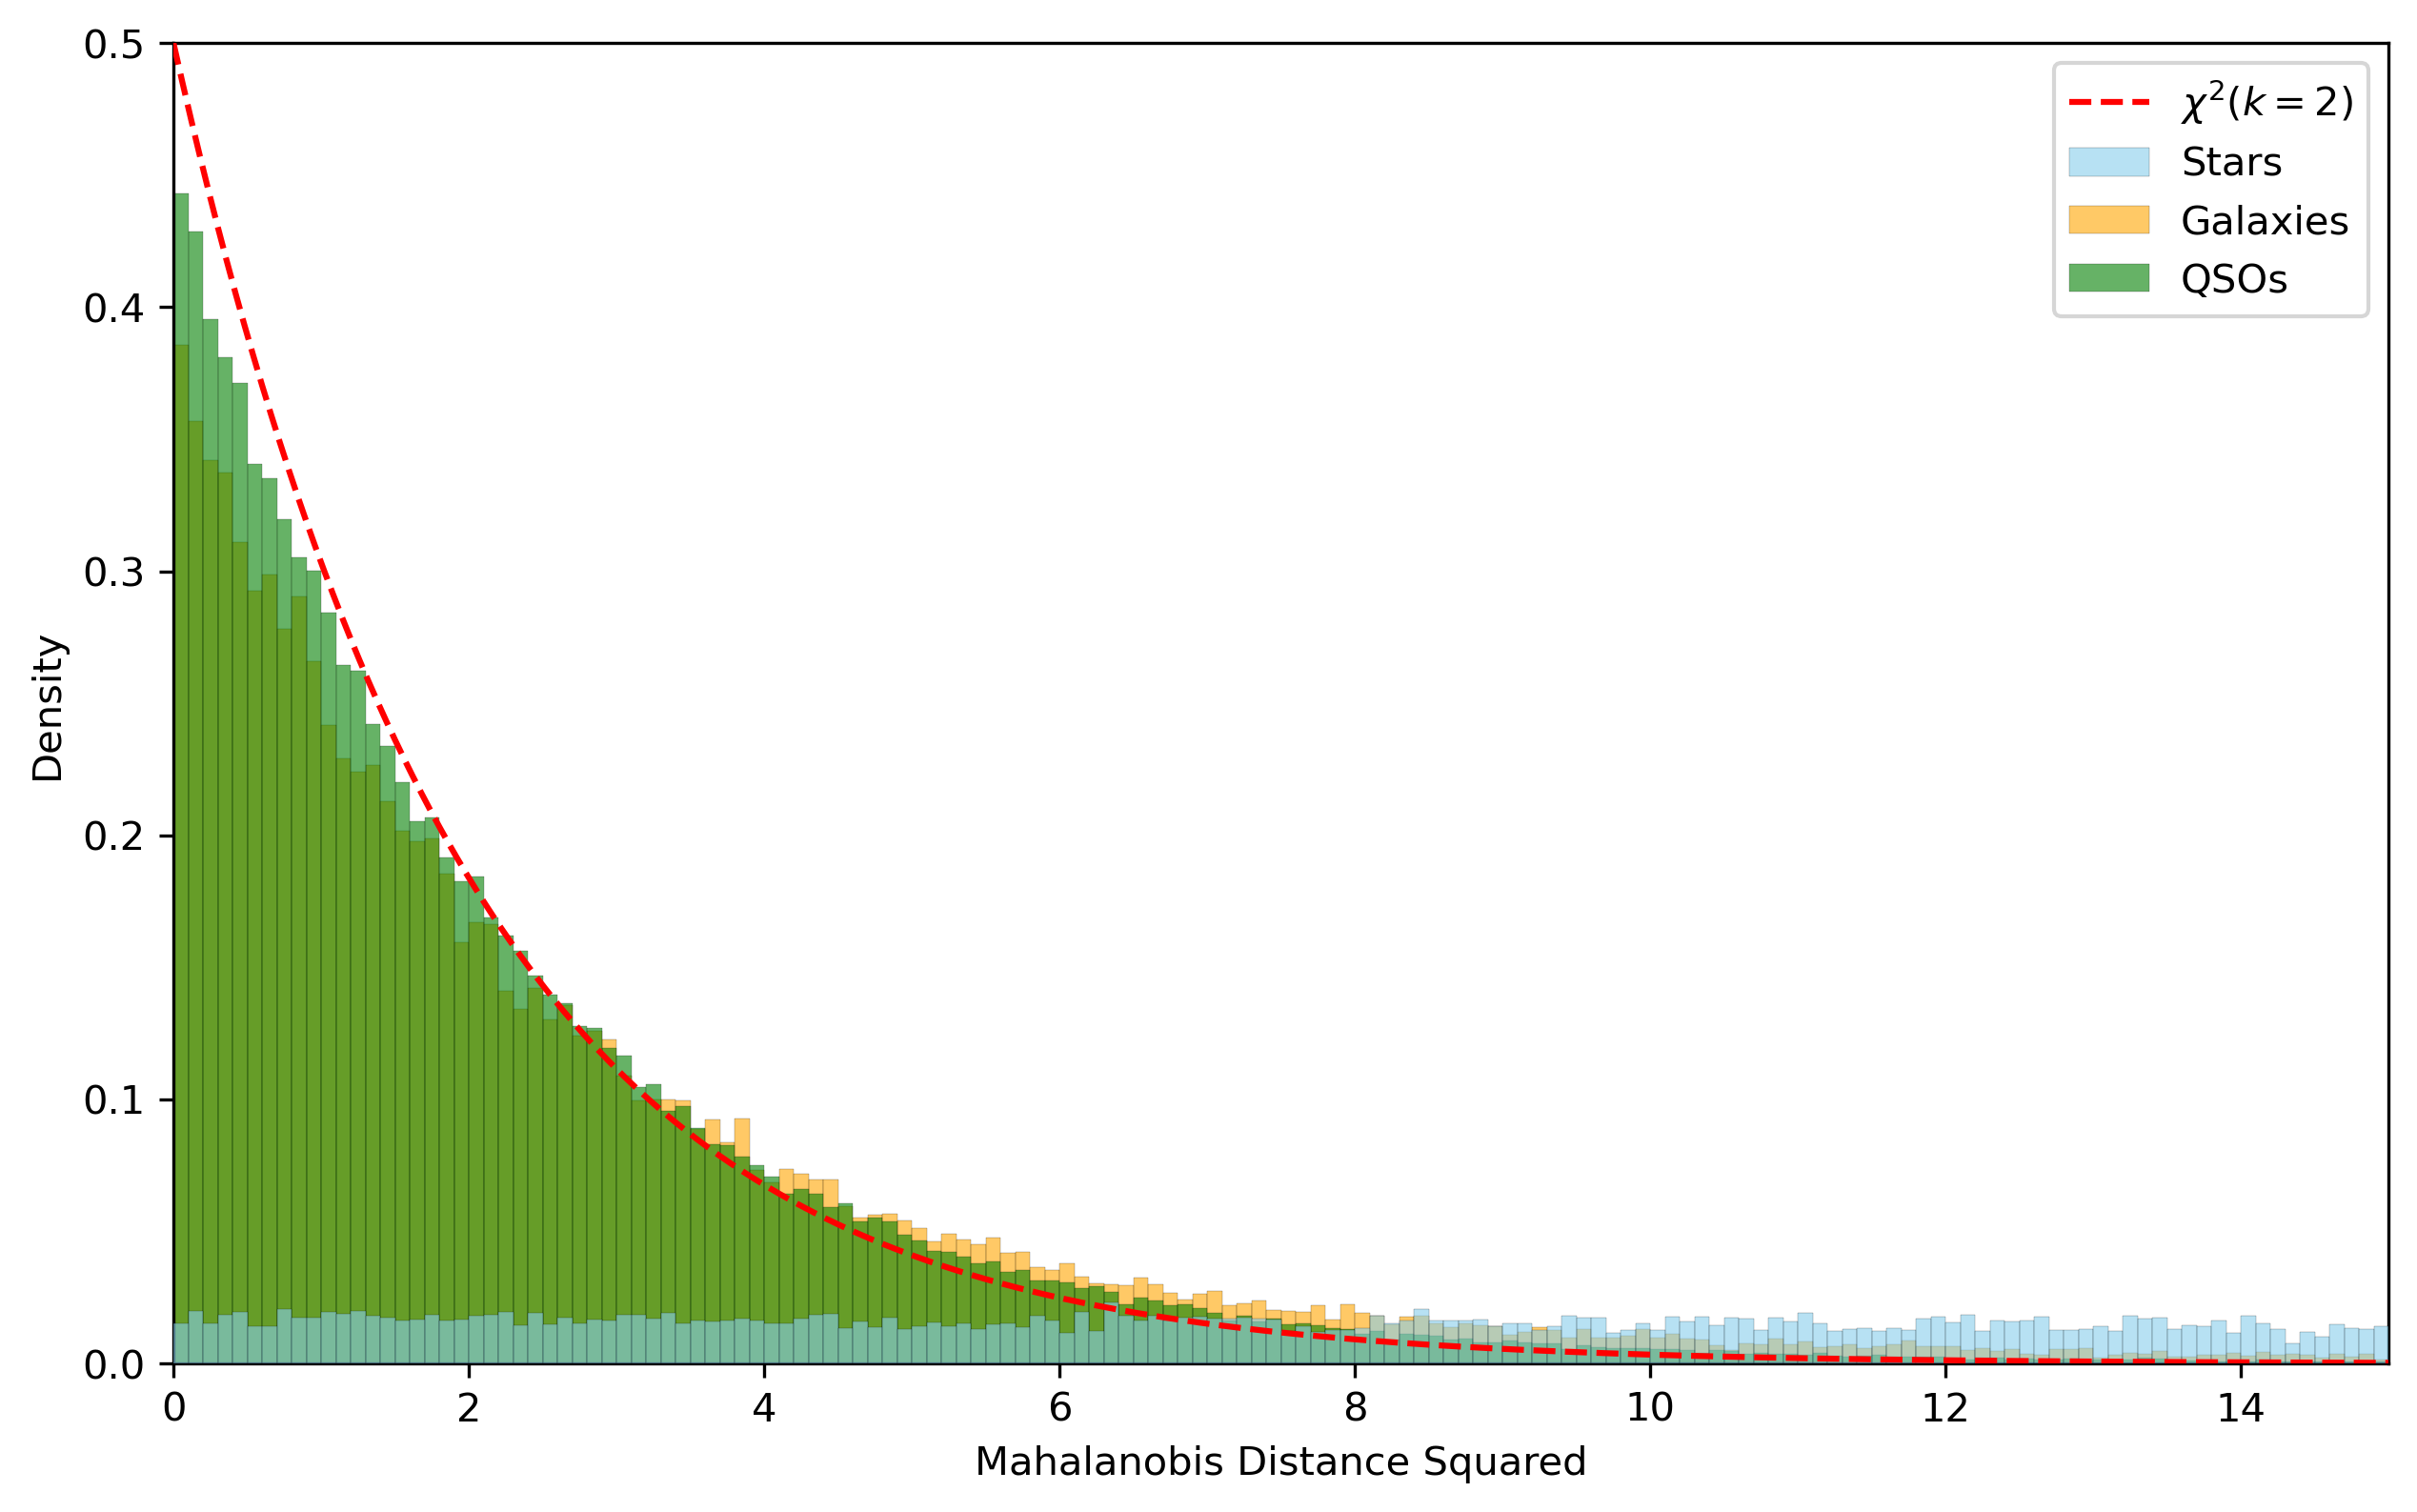
\includegraphics[width=0.9\linewidth]{figs/discuss/m_dist_sq_distribution.png}
    \caption{Squared Mahalanobis Distance of Proper Motion for samples of Quasars, Galaxies and Stars. It's obvious that standard $\chi^2$ distribution can not fit to the practical distribution perfectly.}
    \label{fig:m_dist_sq}
\end{figure}

Therefore, we calculated the $p$-value of the zero proper motion hypothesis using the survival function of the $\chi^2$ distribution. Fig.~\ref{fig:p-value} illustrates the resulting $p$‬-value distributions for the three reference samples.

\begin{figure}[htbp]
    \centering
    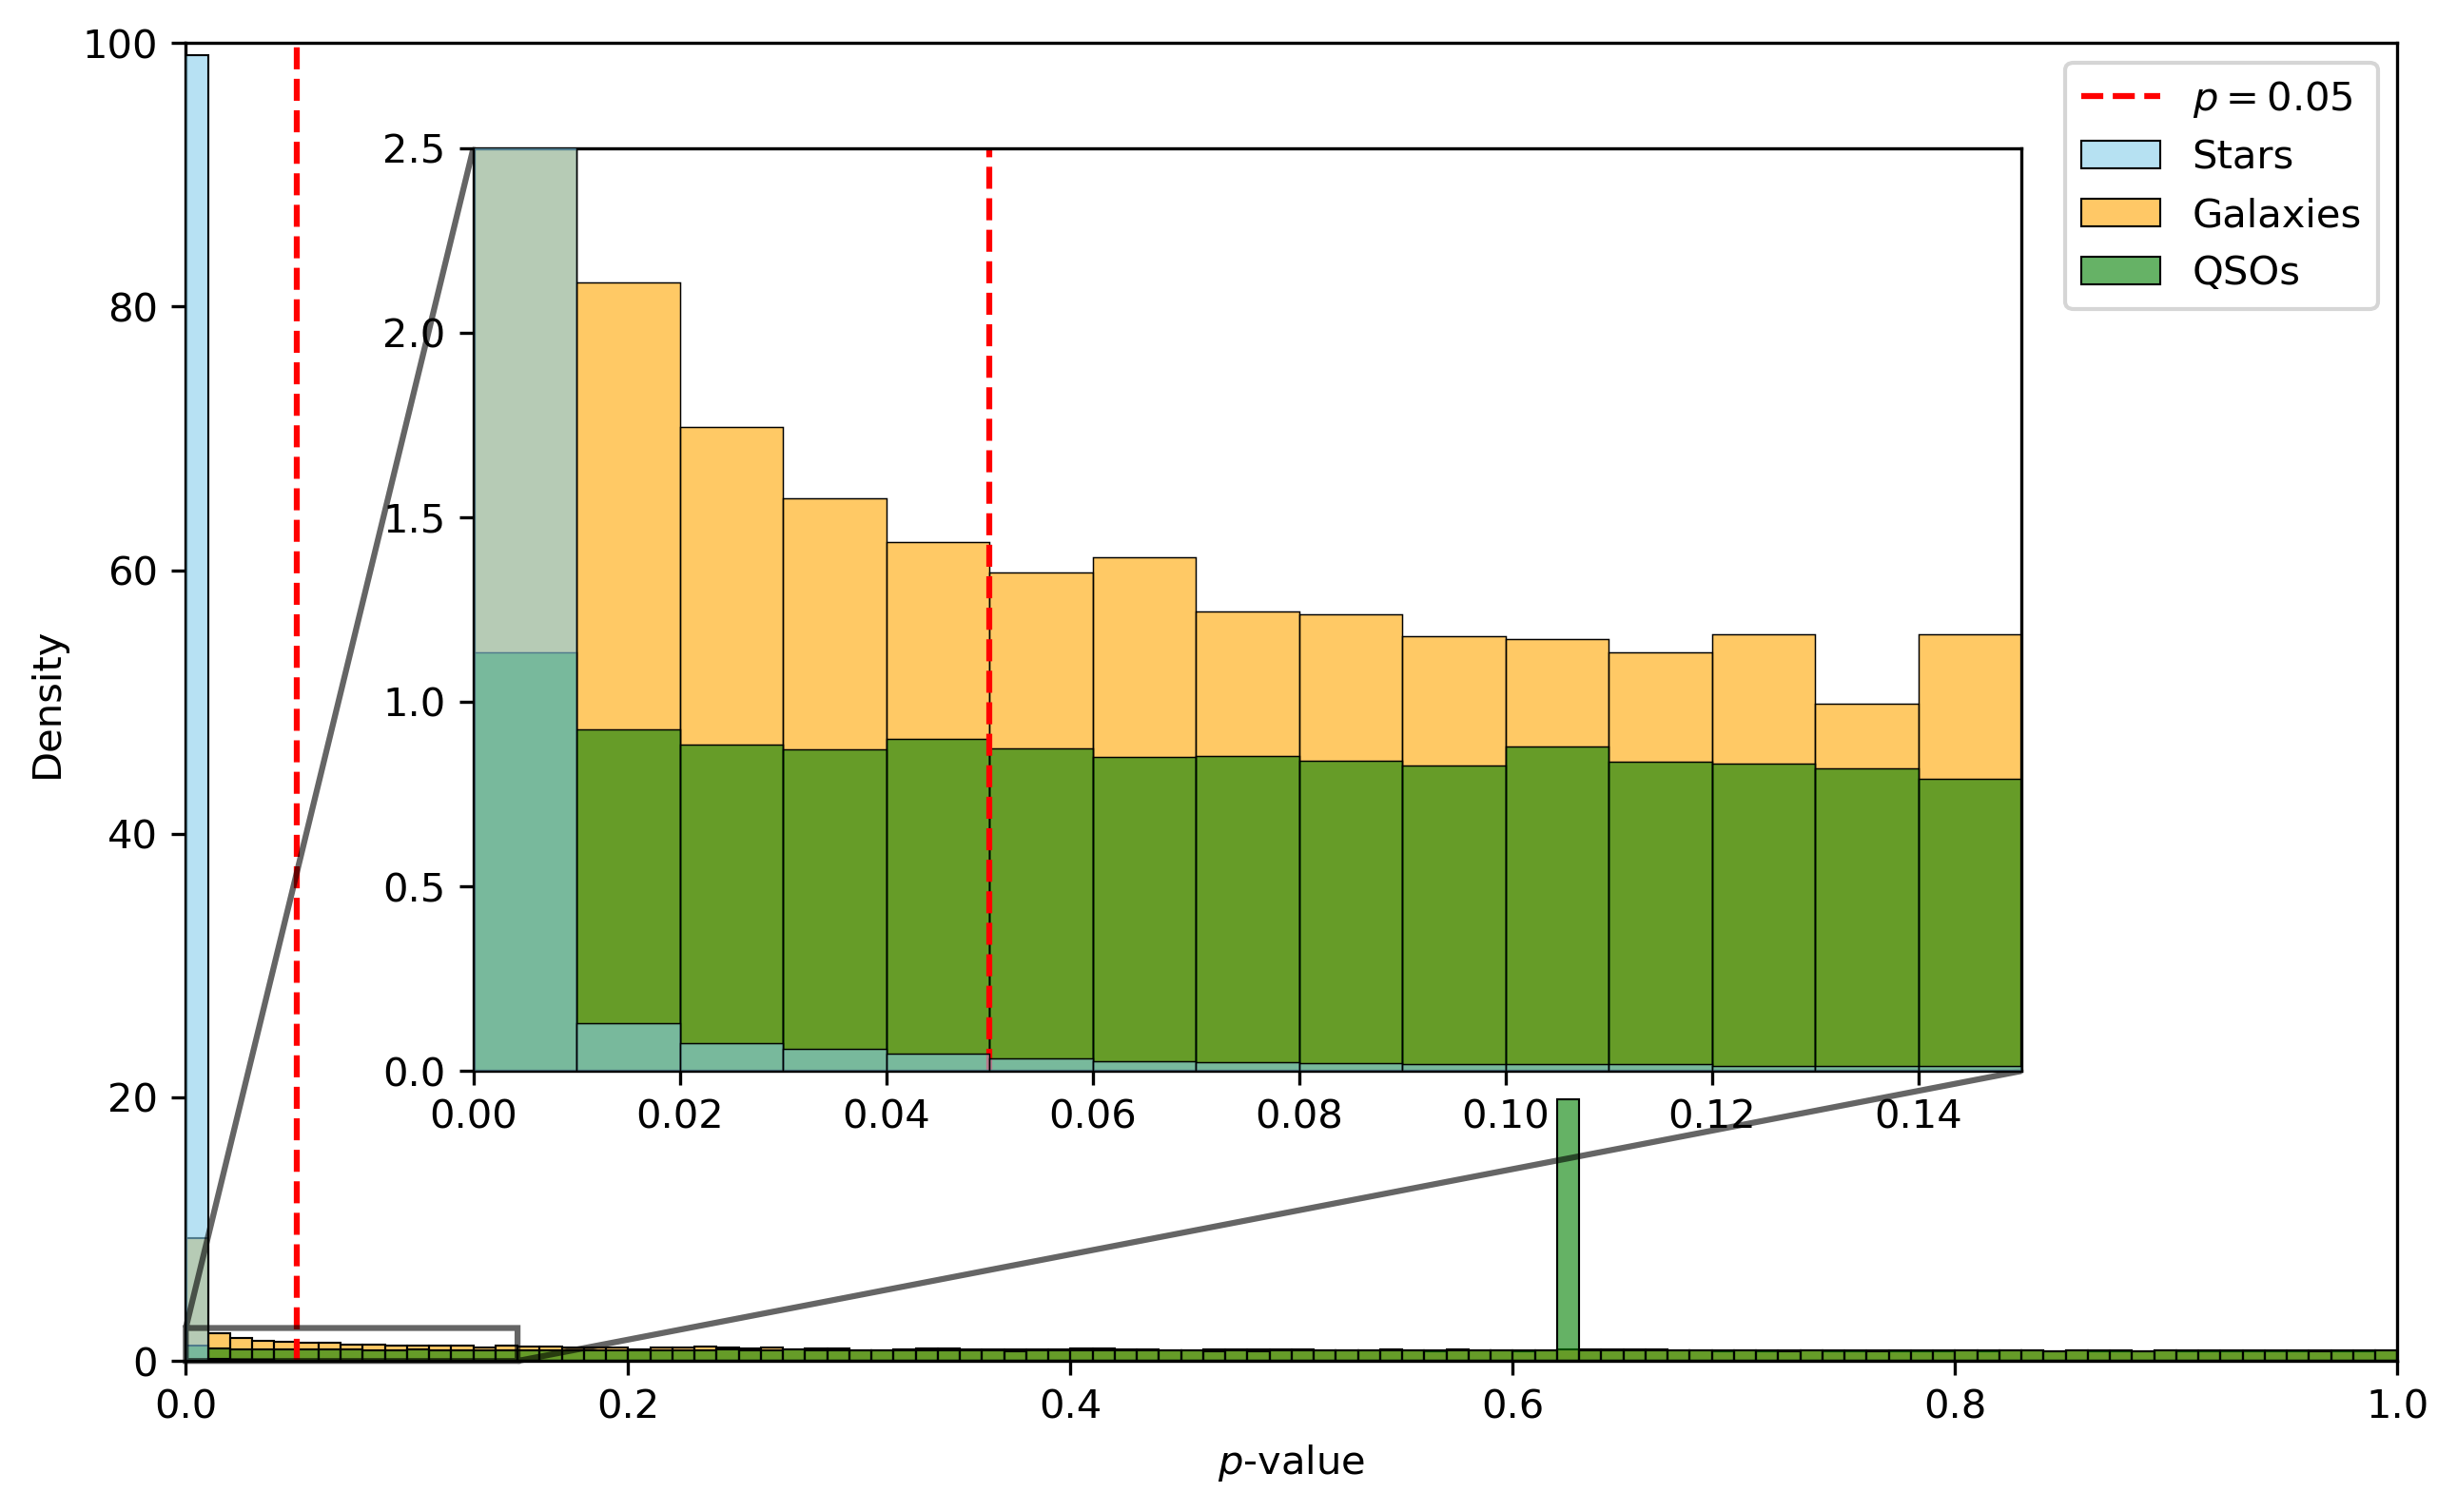
\includegraphics[width=0.9\linewidth]{figs/discuss/sdss_p_zpm_histogram.png}
    \caption{Distributions of $p$-values testing the null hypothesis of zero proper motion ($\boldsymbol{\mu} = (0,0)$) for the quasar, galaxy, and stars samples. The vertical red dashed line indicates the adopted selection threshold at $p=0.05$. The inset panel provides a magnified view of the region $0.00 \leq p \leq 0.15$ to better illustrate the behavior of the distributions near this boundary.}
    \label{fig:p-value}
\end{figure}

For our selection, we adopted a threshold $p=0.05$. This is a conventional significance level in statistical hypothesis testing, roughly corresponding to a $2\sigma$‬‬ confidence interval. The results of applying this selection criterion in reference samples are summarized in Table~\ref{tab:p_res}. 

\begin{table}[htbp]
    \centering
    \begin{tabular}{l l}
    \toprule
    \multicolumn{1}{c}{Sample} & \multicolumn{1}{c}{$p \geq 0.05$} \\
    \midrule
    \textbf{Stars} (SDSS DR17) & $\approx 0.60\%$ (\num{3701} of \num{615304}) \\
    \textbf{Galaxies} (SDSS DR17) & $\approx 83.84\%$ (\num{45305} of \num{54035}) \\
    \textbf{Quasars} (SDSS DR16Q) & $\approx 94.17\%$ (\num{138234} of \num{146794}) \\
    \bottomrule
    \end{tabular}
    \caption{Proportion of $p \geq 0.05$ for Zero Proper Motion in Stars, Galaxies and Quasars Samples.}
    \label{tab:p_res}
\end{table}

In summary, this method successfully rejects $\sim 99.4\%$ of the stars while retaining $\sim 95.3\%$ of the quasars. This retention rate is highly consistent with the theoretical expectation of a $2\sigma$ confidence level ($\sim 95.5\%$). However, because galaxies are also distant extragalactic sources exhibiting zero proper motion, this astrometric criterion alone cannot distinguish them from quasars. To break this degeneracy and remove the remain galaxies as many as possible, we incorporate the \texttt{RUWE} parameter in Gaia Table, as detailed in Section~\ref{sec:ruwe}.

\subsubsection{Optimization for $\chi^2$ Distribution}

As mentioned before, the standard 2 degree-of-freedom $\chi^2$ distribution is not fitted the Squared Mahalanobis Distance distribution of the reference quasar sample. To fix this issue, we applied MAD method to fit the scale parameter of $\chi^2$ distribution to practical distribution. As a result, we find $\mathrm{scale}=1.117$ is the best parameter for the realistic sample, as Figure~\ref{fig:m_fit}.

\begin{figure}[htbp]
    \centering
    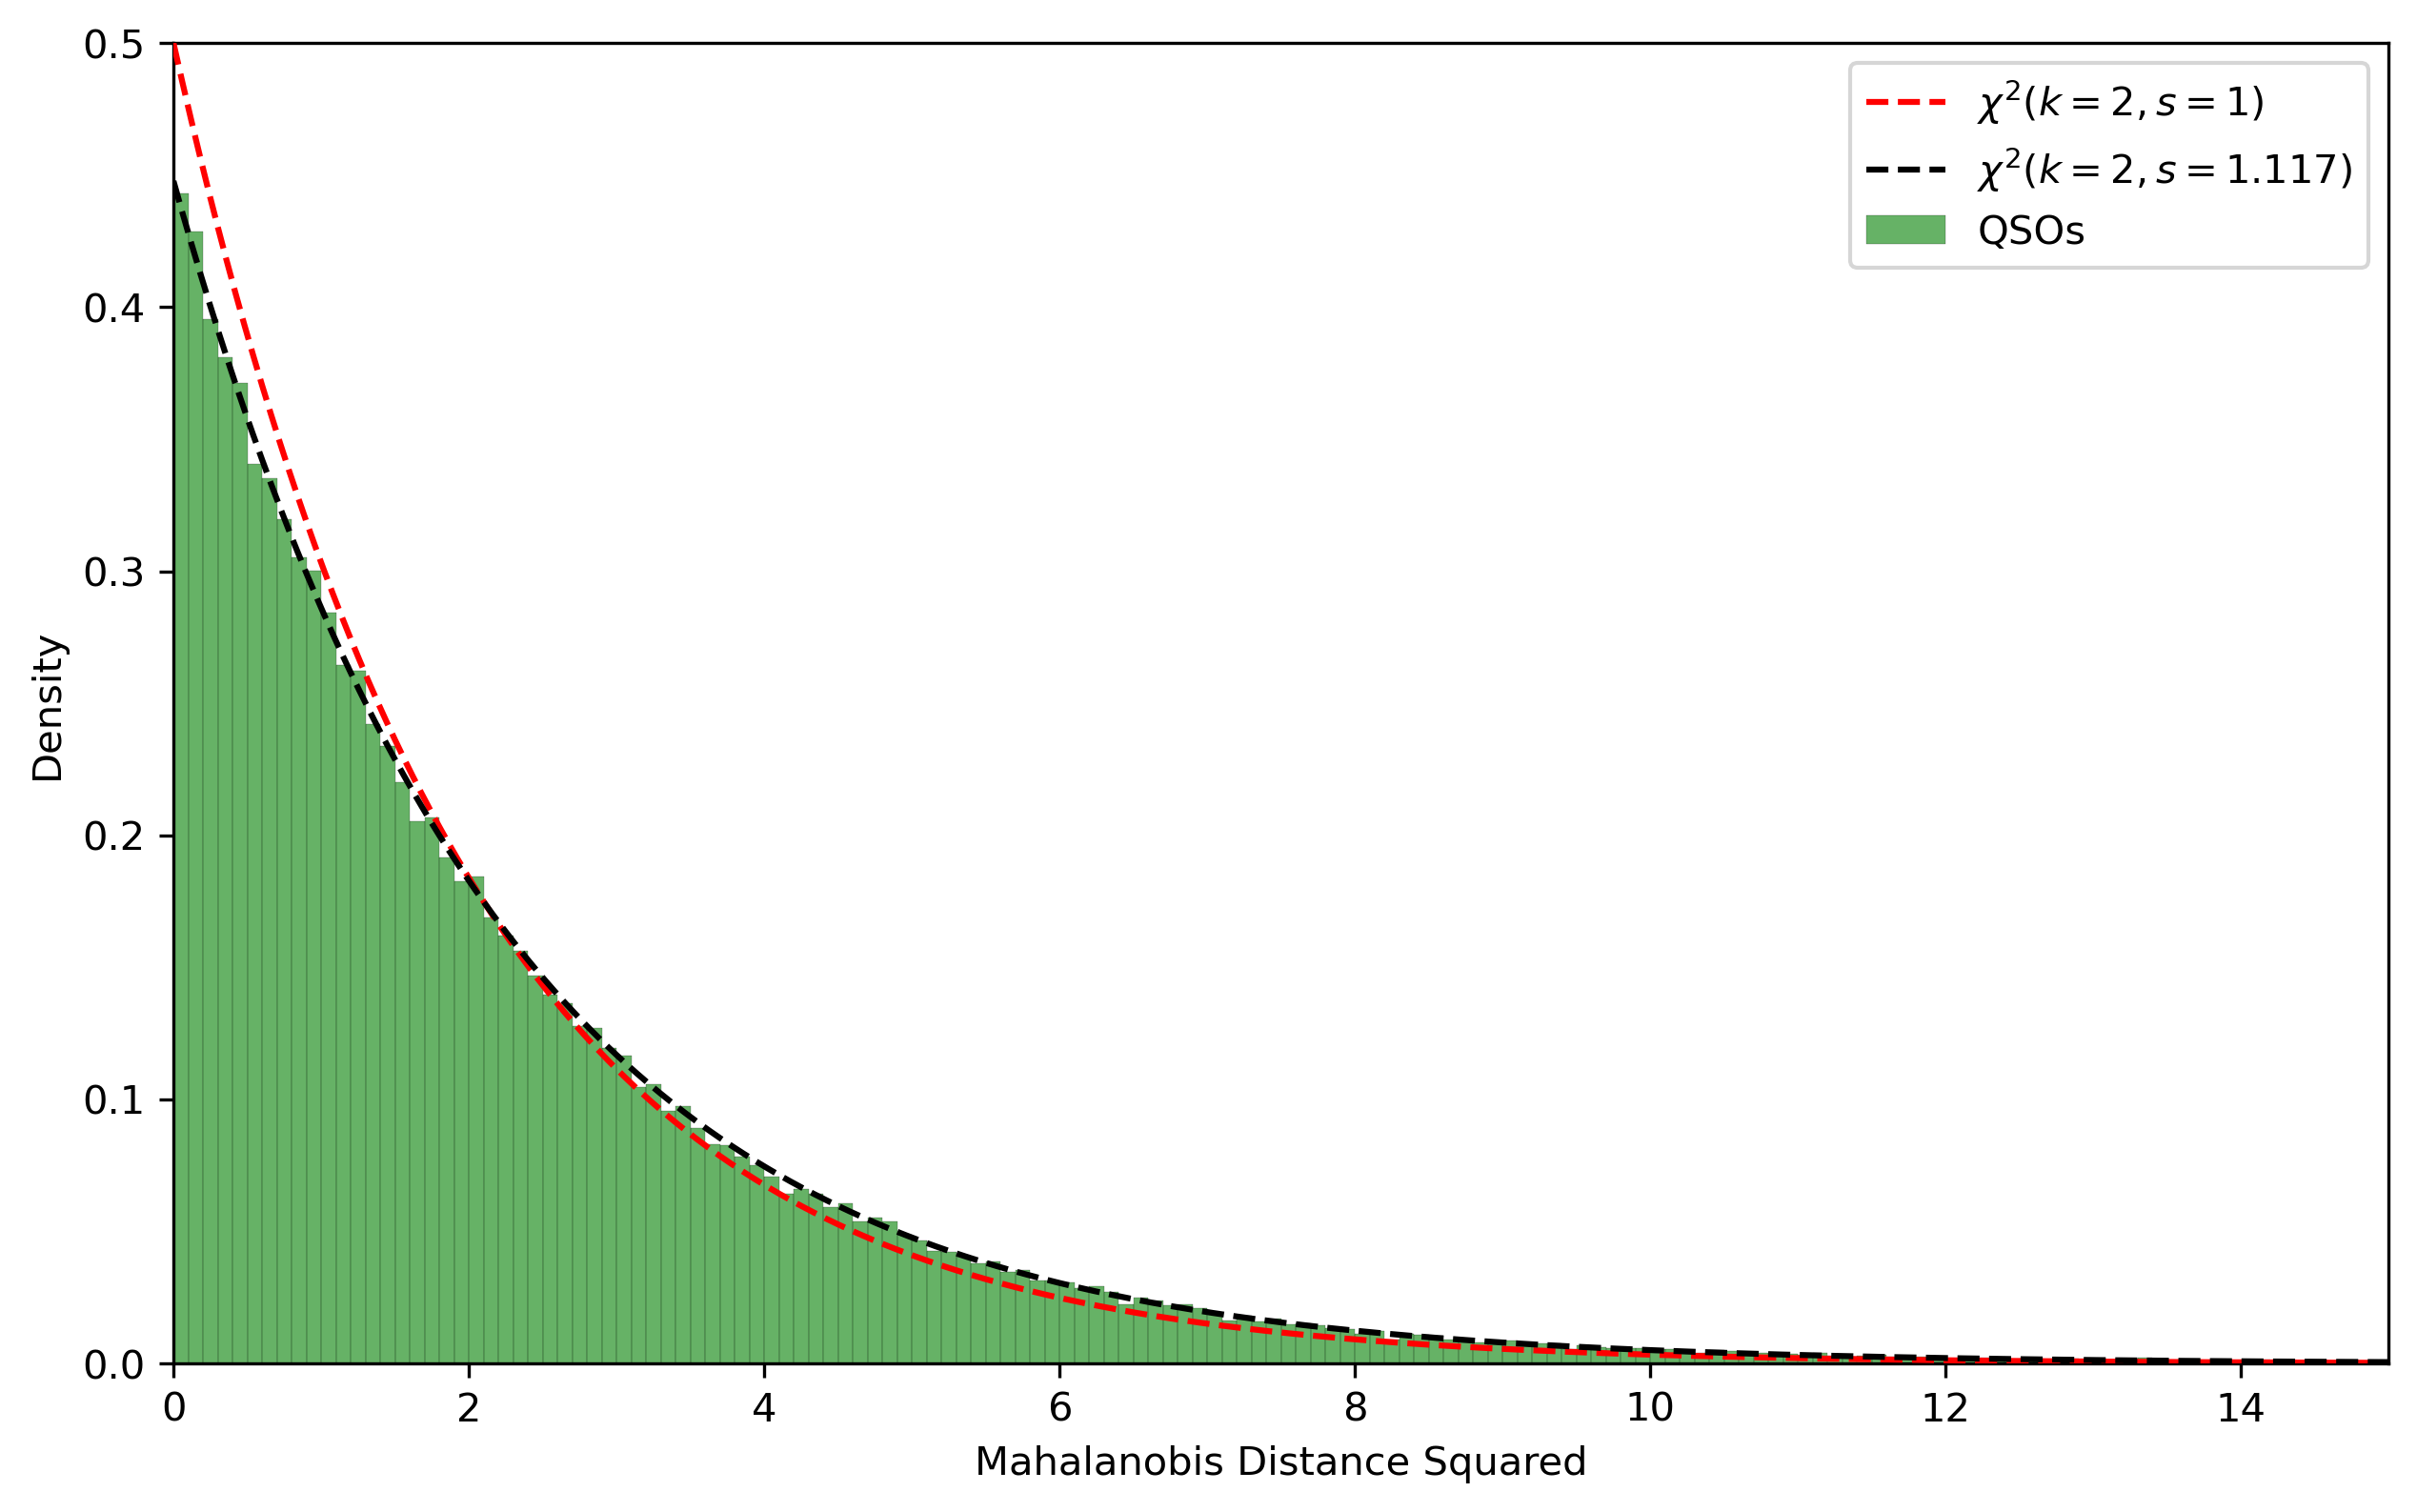
\includegraphics[width=0.9\linewidth]{figs//discuss/m_dist_sq_qso_fit.png}
    \caption{Distributions of $p$-values testing the null hypothesis of zero proper motion ($\boldsymbol{\mu} = (0,0)$) for the quasar sample. The red dashed line is PDF of the standard 2 degree-of-freedom $\chi^2$ distribution and the black dashed line is PDF of fitted distribution with $\mathrm{scale}=1.117$.}
    \label{fig:m_fit}
\end{figure}

As a result, we obtain a new series of $p$-values for the zero proper motion. The comparison between the theoretical distribution and the scaled distribution is summarized in Table~\ref{tab:p_res_fit}.

\begin{table}[htbp]
    \centering
    \begin{tabular}{l l l}
    \toprule
    \multicolumn{1}{c}{Sample} & \multicolumn{1}{c}{$p \geq 0.05$} & \multicolumn{1}{c}{$p \geq 0.05$ ($\mathrm{scale}=1.117$)} \\
    \midrule
    \textbf{Stars} (\num{615304}) & $\approx 0.60\%$ (\num{3701}) &  $\approx 0.67\%$ (\num{4149}) \\
    \textbf{Galaxies} (\num{54035}) & $\approx 83.84\%$ (\num{45305}) &  $\approx 86.02\%$ (\num{46482}) \\
    \textbf{Quasars} (\num{146794}) & $\approx 94.17\%$ (\num{138234}) &  $\approx 94.70\%$ (\num{139021}) \\
    \bottomrule
    \end{tabular}
    \caption{The Comparison of Proportion of $p \geq 0.05$ for Zero Proper Motion in Stars, Galaxies and Quasars Samples. The scale parameter has a negligible impact on the final selection results.}
    \label{tab:p_res_fit}
\end{table}

It is evident that the variation in the scale parameter has a negligible impact on the final selection results. Consequently, we continue to employ the standard $\chi^2$‬ distribution for the remainder of this analysis.

\subsection{\texttt{RUWE} in Gaia DR3}
\label{sec:ruwe}

The Gaia archive provides the \textbf{Renormalised Unit Weight Error} (\texttt{ruwe}) as a crucial indicator to evaluate the quality of the astrometric solutions. This statistic is mathematically defined as:
\begin{equation}
    \text{ruwe} = \frac{\sqrt{ \chi^2_{\text{AL}} / (N_{\text{good,AL}} - m) }}{f(G, G_{\text{BP}-\text{RP}})},
    \label{eq:ruwe}
\end{equation}
where $\chi^2_{\text{AL}}$ represents the astrometric goodness-of-fit (\texttt{astrometric\_chi2\_al}) in the along-scan (AL) direction, and $N_{\text{good,AL}}$ is the number of good AL observations (\texttt{astrometric\_n\_good\_obs\_al}). The variable $m$ denotes the number of astrometric parameters solved, which is derived from the number of set bits in the \texttt{astrometric\_params\_solved} parameter. The denominator, $f(G, G_{\text{BP}-\text{RP}})$, is determined in an off-line statistical analysis of the secondary solutions \citep{vanleeuwenGaiaDR3Documentation2022,lindegrenGaiaEarlyData2021}. This parameter $f$ is a statistical results to mitigate systematic biases associated with a source's $G$-band magnitude and colour \citep{Lindegren2018RUWE}.

For well-behaved point sources, the \texttt{ruwe} value is theoretically expected to be around 1.0. At the same time, galaxies are spatially extended sources, which means their astrometric fits in Gaia are typically poorer than those of point-like quasars, resulting in elevated \texttt{ruwe} values. Consequently, the \texttt{ruwe} parameter serves as an effective discriminant \citep{gaiacollaborationGaiaDataRelease2023a}. Figure~\ref{fig:ruwe} illustrates the \texttt{RUWE} distributions for the quasar, galaxy, and stellar reference samples.

\begin{figure}[htbp]
    \centering
    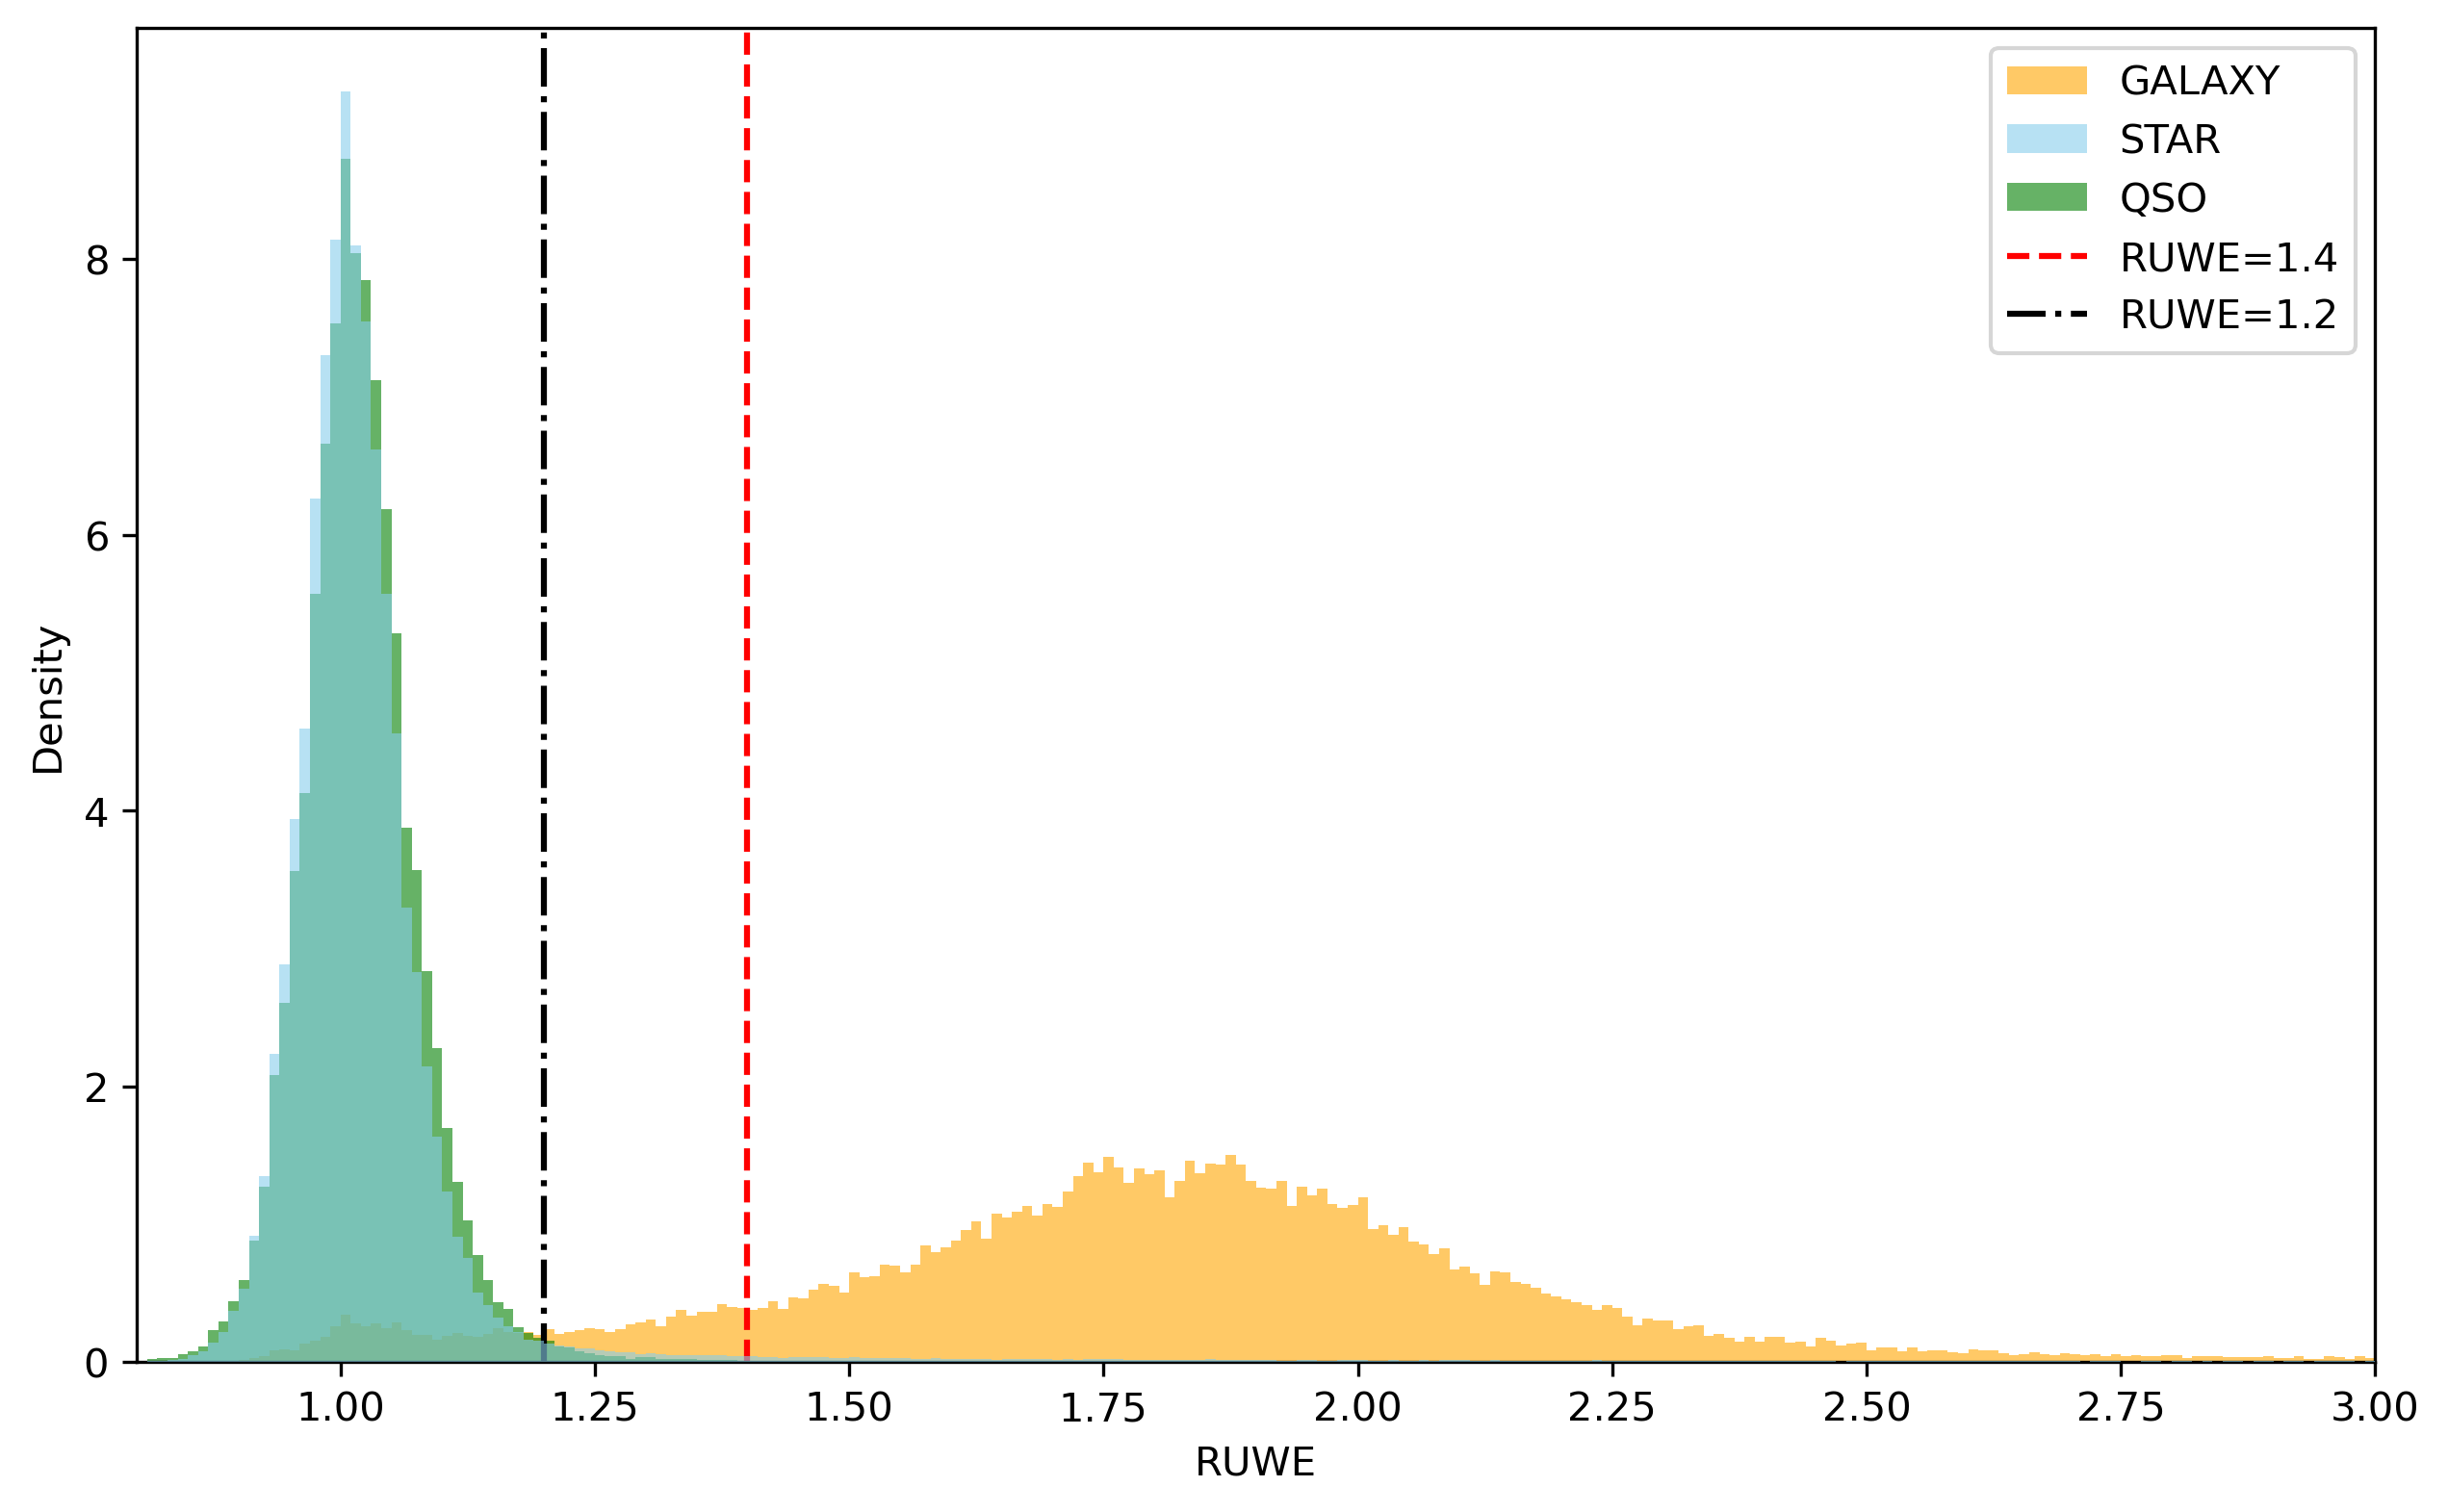
\includegraphics[width=0.9\linewidth]{figs//discuss/RUWE_distribution.png}
    \caption{\texttt{ruwe} Distribution in Stars, Galaxies and Quasars Samples. It illustrate that the \texttt{ruwe} of point sources are normally around 1. At the same time, the galaxies usually have a higher \texttt{ruwe}.}
    \label{fig:ruwe}
\end{figure}

To determine the better threshold of \texttt{ruwe} in our selection, we chose two values to compare the effect. The threshold $\mathrm{ruwe}<1.4$ is widely used in multiple papers such as \citet{fabriciusGaiaEarlyData2021} to remove potential non-single objects, and $\mathrm{ruwe}<1.2$ represents the same density level in the distribution of three reference samples. The comparison results are shown in Table~\ref{tab:ruwe}.

\begin{table}[htbp]
    \centering
    \begin{tabular}{l l l}
    \toprule
    \multicolumn{1}{c}{Sample} & \multicolumn{1}{c}{$\mathrm{ruwe} < 1.4$} & \multicolumn{1}{c}{$\mathrm{ruwe} < 1.2$} \\
    \midrule
    \textbf{Stars} (\num{615304}) & $\approx 96.86\%$ (\num{595983}) &  $\approx 95.43\%$ (\num{587169}) \\
    \textbf{Galaxies} (\num{54035}) & $\approx 11.58\%$ (\num{6259}) &  $\approx 5.66\%$ (\num{3057}) \\
    \textbf{Quasars} (\num{146794}) & $\approx 99.78\%$ (\num{146469}) &  $\approx 98.88\%$ (\num{139021}) \\
    \bottomrule
    \end{tabular}
    \caption{The Comparison of different thresholds of \texttt{ruwe} in Stars, Galaxies and Quasars Samples.}
    \label{tab:ruwe}
\end{table}

Ultimately, we adopt the condition $\mathrm{ruwe} < 1.4$ to strike an optimal balance between filtering out galactic contaminants and retaining a maximal number of quasar candidates, as demonstrated in Table~\ref{tab:ruwe}.

\subsection{Selection Result and Validation}

Based on the preceding discussions, our updated selection criteria are summarized as follows:
\begin{itemize}
    \item In SNAQS footprint (RA: \qtyrange{190}{210}{\degree}, Dec: \qtyrange{22}{36}{\degree})
    \item Brighter than 19  Magnitude in Gaia G-band ($m_G<19$)
    \item Parallax is zero in $2\sigma$ ($\varpi/\sigma_{\varpi}<2$)
    \item $p$-value of zero proper motion is larger than $0.05$ ($p_{\mathrm{zpm}}\geq0.05$)
    \item \texttt{ruwe} is lower than 1.4 ($\mathrm{ruwe}<1.4$)
\end{itemize}
Applying these combined criteria yields a final updated sample comprising \num{1794} sources. 

To validate the superior performance of our updated selection criteria, we employ the SDSS DR16 quasar catalogue (DR16Q) as a reference sample. We cross-matched the DR16Q catalogue with Gaia DR3 using a \qty{1}{\arcsecond} matching radius, isolating all visually confirmed quasars (including standard quasars, BAL quasars, and blazars) brighter than $m_G = 19$ within the SNAQS footprint. By evaluating the recovery rate of these confirmed quasars across both selection methods, we demonstrate the efficiency of our new method. The results are summarized in Table~\ref{tab:sdss_dr16q_comp}. It shows the new selection has a better performance.

\begin{table}[htbp]
    \centering
    \begin{tabular}{c c c}
    \toprule
    Sample & Old Selection & New Selection \\
    \midrule
    \textbf{SDSS DR16Q} (\num{464}) & $\approx 77.16\%$ (\num{358}) & $\approx 91.38\%$ (\num{424}) \\
    \bottomrule
    \end{tabular}
    \caption{Comparison of the quasar completeness rates using the SDSS DR16Q reference catalogue. The results indicate that the updated selection method achieves a significantly higher completeness for known quasars.}
    \label{tab:sdss_dr16q_comp}
\end{table}

Furthermore, we cross-matched our two selection samples with the SDSS DR19, LAMOST DR11, and DESI DR1 catalogues using a \qty{1}{\arcsecond} matching radius. The resulting classifications for each survey are summarized in Table~\ref{tab:survey_comparison}.\footnote{Note that these classifications rely entirely on automated pipeline outputs and have not been visually verified.\label{fn:auto_pipeline}}

\begin{table}[htbp]
    \centering
    \begin{tabular}{l l c c}
        \toprule
        \textbf{Survey} & \textbf{Type} & \textbf{Old Selection} & \textbf{New Selection} \\
        \midrule
        \multirow{3}{*}{\textbf{SDSS DR19}} 
        & QSO    & \num{1271} ($\approx 88.63\%$) & \num{1518} ($\approx 97.87\%$) \\
        & Galaxy & \num{159} ($\approx 11.09\%$) & \num{28} ($\approx 1.81\%$) \\
        & Star   & \num{4} ($\approx 0.28\%$) & \num{5} ($\approx 0.32\%$) \\
        \midrule
        \multirow{3}{*}{\textbf{LAMOST DR11}} 
        & QSO    & \num{609} ($\approx 85.77\%$) & \num{724} ($\approx 94.03\%$) \\
        & Galaxy & \num{81} ($\approx 11.41\%$) & \num{22} ($\approx 2.86\%$) \\
        & Star   & \num{20} ($\approx 2.82\%$) & \num{24} ($\approx 3.11\%$) \\
        \midrule
        \multirow{3}{*}{\textbf{DESI DR1}} 
        & QSO    & \num{675} ($\approx 85.88\%$) & \num{796} ($\approx 93.87\%$) \\
        & Galaxy & \num{103} ($\approx 13.10\%$) & \num{39} ($\approx 4.60\%$) \\
        & Star   & \num{8} ($\approx 1.02\%$) & \num{13} ($\approx 1.53\%$) \\
        \bottomrule
    \end{tabular}
    \caption{Comparison of the classification results between the old and new selection methods across SDSS, LAMOST and DESI catalogues. \textsuperscript{\ref{fn:auto_pipeline}}}
    \label{tab:survey_comparison}
\end{table}

Consequently, we evaluate the number of confirmed quasars in both selections. A source is designated as a confirmed quasar if it is spectroscopically classified as a 'QSO' in at least one of the SDSS~DR19, LAMOST~DR11 or DESI~DR1 catalogues.\textsuperscript{\ref{fn:auto_pipeline}} After merging these records from other surveys with the SNAQS observational results and removing duplicate entries, we determine the final quasar fraction for both selection methods, as presented in Table~\ref{tab:qso_prob}.
\begin{table}[htbp]
    \centering
    \begin{tabular}{c c c}
        \toprule
         & Old Selection & New Selection \\
        (Observed Targets) & (\num{1582}) & (\num{1715}) \\
        \midrule
        \textbf{Quasars} & \num{1388} ($\approx 87.74\%$) & \num{1649} ($\approx 96.15\%$) \\
        \bottomrule
    \end{tabular}
    \caption{The quasar fraction for both selection methods. The results demonstrate that the updated criteria achieve a significantly higher purity of quasar candidates.\textsuperscript{\ref{fn:auto_pipeline}}}
    \label{tab:qso_prob}
\end{table}

In conclusion, our updated method demonstrates superior performance for the purely astrometric selection of quasar candidates. Most notably, it successfully elevates the overall quasar purity to the $2\sigma$ level ($\sim 95\%$).

\section{Some Other Issue in SNAQS}

\subsection{Additional Issues in Quasars Selection}

Beyond our discussion above, there are some other issues that may influence the features of astrometric data for quasars. Such as \citet{gaiacollaborationGaiaEarlyData2021} found a systematic \qty{\sim5}{\mu as/yr} proper motion of background objects (like quasars) due to the acceleration of the solar system. Unresolved double or multiple AGNs may also cause some quasars to seem as if they have proper motion in the optical band \citep{makarovQuasarsProperMotions2022}. The quasars' variability is another potential reason for why they are measured with proper motion \citep{bachchanGaiaReferenceFrame2016}. 

In a nutshell, we still need more time on research to understand this mysterious type of objects.

\subsection{Potential Stars in Our Selection}

Based on previous discussion, our selection still contains some stars. These stars are far from the galaxy disk because our selection is aim to find distant targets near galactic polars. Like \textbf{SDSS~J131310.5$+$232833.9} and \textbf{SDSS~J132035.7$+$340814.6} which are mentioned in previous chapter, they are potential valuable in galactic archaeology \citep{freemanNewGalaxySignatures2002}.

\section{A Special Case in SDSS DR16Q}

We also found a special source in the SDSS Quasar Catalog: DR16 \citep{lykeSloanDigitalSky2020}, \textbf{SDSS~J135757.63$+$295418.5}. This object is marked as quasar by automatic pipeline but not be visually verified. Figure~\ref{fig:hig_pm_sdss} is the spectrum of this target.

\begin{figure}[htbp]
    \centering
    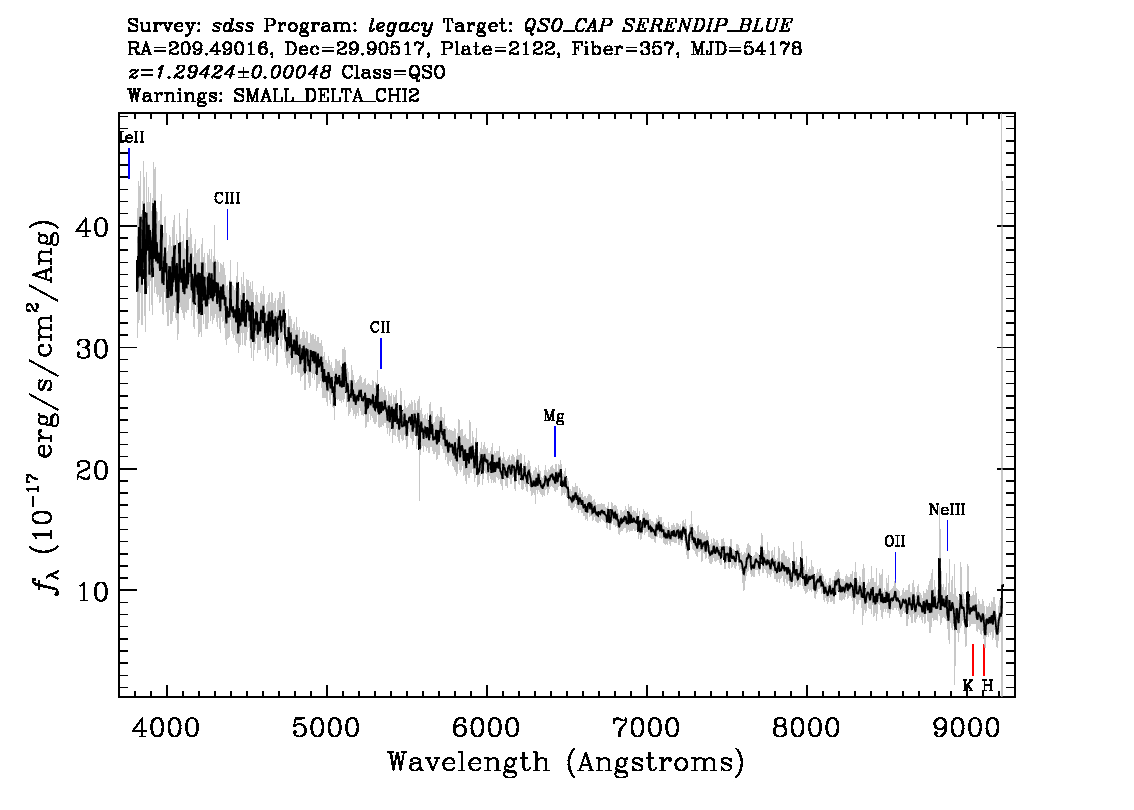
\includegraphics[width=1\linewidth]{figs//discuss/SpecById.ashx.png}
    \caption{Spectrum of \textbf{SDSS~J135757.63$+$295418.5} from SDSS DR19 \citep{collaborationNineteenthDataRelease2025}. We prefer this is a White Dwarf.}
    \label{fig:hig_pm_sdss}
\end{figure}

But in Gaia DR3, this object has a very high parallax and proper motion for a quasar. The parallax is \qty{\sim12.60}{mas} ($\sim118\sigma$ from 0) and total proper motion is \qty{22.99}{mas/yr}. If we use $z=1.29$ (as in SDSS DR16Q) to calculate its move speed, the value will be multiple times of light speed, which is impossible in physics. In conclusion, with the photometric data, we think this object is high probability as a white dwarf in the galaxy.

In Gaia DR2 \citep{gaiacollaborationGaiaDataRelease2018}, while the parallax of this object is similar (\qty{\sim12.69}{mas}), the uncertainty of parallax is much higher, made the parallax is only $\sim0.5\sigma$ from 0. At the same time, the proper motion also has this condition. This is a potential reason why it is still in the quasar catalogue.

Furthermore, this object also made some interesting error. The automatic classifier of Gaia mission is based on machine learning \citep{vanleeuwenGaiaDR3Documentation2022}, and they used SDSS DR16Q as a training dataset for quasars. Consequently, this object became the contamination in training.

Also, this case demonstrate that the accuracy of the selection based on astrometry will be increased as the precision of astrometric measurements improvement.
